\documentclass[fleqn,usenatbib]{mnras}
\usepackage{amsmath,amssymb}
\usepackage{graphicx}
\usepackage{booktabs,tabularx,array}
\usepackage{xcolor}
\usepackage{hyperref}
\hypersetup{hidelinks}
\graphicspath{{figures/}}
\newcolumntype{L}{>{\raggedright\arraybackslash}X}
\newcommand{\papertablestyle}{\footnotesize\setlength{\tabcolsep}{4pt}\renewcommand{\arraystretch}{1.1}}

\title[Magnification of lensed gravitational waves]{How well can the magnification of a strongly lensed gravitational wave be measured? A benchmark with GWTC-4.0 populations and O4a noise}
\author[Zhang et al.]{Fan Zhang,$^{1,2}$ Junxiao Kong,$^{1,3}$ Qikai Zhang,$^{1}$ Qiyuan Yang,$^{4}$ Shaohan Wei,$^{3}$ and Xilong Fan$^{4}$\thanks{E-mail: xilong.fan@whu.edu.cn}\\
$^{1}$State Key Laboratory of Ocean Sensing and Ocean College, Zhejiang University, Zhoushan 316021, China\\
$^{2}$Kavli Institute for Astrophysics and Space Research, Massachusetts Institute of Technology, Cambridge, MA 02139, USA\\
$^{3}$School of Mathematics and Statistics, Lanzhou University, Lanzhou 730000, China\\
$^{4}$School of Physics and Technology, Wuhan University, Wuhan 430072, China}
\date{Accepted XXX. Received YYY; in original form ZZZ}
\pubyear{2026}

\begin{document}
\label{firstpage}
\pagerange{\pageref{firstpage}--\pageref{lastpage}}
\maketitle

\begin{abstract}
Correcting the luminosity distance of a strongly lensed gravitational-wave (GW) source requires the absolute magnification of its images, which GW data alone cannot measure. We quantify how accurately and how reliably it can be obtained by combining GW signals with an electromagnetic model of the lens galaxy. We simulate $8\times10^5$ lensed binary black holes from the GWTC-4.0 population, four galaxy-lens models from the singular isothermal sphere (SIS) to the elliptical power law with external shear, and an O5-like network and the Einstein Telescope (ET), with GW distance errors calibrated on 167 GWTC events. Using only observables that are unaffected by the mass-sheet degeneracy and contain no distance scale---the image positions relative to the lens light, the GW relative magnification and the image arrival order---estimators trained on the simulations determine the magnification of an ET image to a median 3, 7, 10 and 19 per cent for the four lens models (O5: 10--27 per cent). Adding the time delay and redshifts lowers the errors further, but only because the estimator learns the simulated cosmology. Near caustics the errors grow roughly in proportion to the magnification, and the 90 per cent intervals contain the true value for only about half of the images with $\mu>20$. An SIS lens prior gives confidently wrong intervals for realistic lenses, whereas calibrating on elliptical power-law lenses gives reliable intervals for all lens models at 40 per cent greater width. Bayesian parameter estimation of 120 lensed pairs from simulated detector data confirms the GW error model, and a conventional Bayesian lens reconstruction of the same systems reaches 8 (ET) and 14 (O5) per cent, comparable to the trained estimators; its fast two-step version agrees with the full analysis of the detector data. Positional errors of 0.1\,arcsec for the GW images in the host double the magnification error. All results assume reconstructed image positions of the GW source within the host and no external mass sheet.
\end{abstract}

\begin{keywords}
gravitational lensing: strong -- gravitational waves -- methods: data analysis -- methods: statistical
\end{keywords}

\section{Introduction}
\label{sec:introduction}
Strong gravitational lensing by intervening galaxies splits a gravitational-wave (GW) signal into several images that arrive with relative delays of minutes to months, with different magnifications and with discrete Morse phase shifts \citep{takahashi2003waveeffects,dai2017morse,ezquiaga2021phase}. Current detectors are expected to observe roughly one strongly lensed binary-black-hole (BBH) pair per thousand detections, rising to hundreds of pairs per year for third-generation instruments such as the Einstein Telescope \citep[ET;][]{ng2018rates,li2018statistical,oguri2018distribution,wierda2021beyond}. Searches of the LIGO--Virgo--KAGRA (LVK) data through the fourth observing run have not yet produced a confident multiple-image detection \citep{hannuksela2019search,lvk2021o3a,lvk2024o3search,lvk2025gwtc4lensing}, but the rapidly growing catalogue \citep{lvk2025gwtc4} makes the first detections a realistic near-term prospect.

A lensed GW image has strain amplitude proportional to $\sqrt{|\mu|}/d_L$, where $\mu$ is its signed magnification and $d_L$ the luminosity distance of the source. GW data alone therefore measure only the apparent distance $d_L/\sqrt{|\mu|}$ of each image and the \emph{relative} magnifications between images. Correcting the luminosity distance---for cosmography, tests of GW propagation or population studies \citep{liao2017precision,oguri2019review}---requires the \emph{absolute} magnification of at least one image. This in turn requires a lens model, which must be constrained by electromagnetic (EM) observations of the lens and of the lensed host galaxy \citep{hannuksela2020localizing,wempe2022lensing,smith2023discovering,uronen2026galacticcentres}. The mass-sheet degeneracy \citep{falco1985msd,schneider2013msd} implies that no combination of image positions and flux ratios can fix the absolute magnification without an assumption about, or a measurement of, the external convergence.

Combining GW relative magnifications and time delays with an EM reconstruction of the lens to obtain absolute magnifications and source distances is not new. \citet{hannuksela2020localizing} demonstrated the principle, including the distance reconstruction, for representative systems. \citet{wempe2022lensing} studied the joint GW and EM selection and host localisation of lensed BBHs. \citet{poon2025degeneracy} derived which lens and source quantities GW lensing can identify and how the mass-sheet and similarity degeneracies enter. \citet{uronen2026silmarel} built a joint Bayesian reconstruction framework that adds Gaussian likelihood terms for the GW relative magnifications and delays to an EM lens model, and \citet{uronen2026galacticcentres} applied this approach to locating BBHs within their hosts. What has not been established is how accurate and how \emph{reliable} absolute-magnification estimates are across realistic lens and source populations: when the quoted uncertainty can be trusted, when it is set by the prior rather than the data, and when it fails. Magnification benchmarks of this kind exist for cluster lenses \citep{meneghetti2017ff}, but not for galaxy-scale lensed GWs.

This paper provides such a benchmark. We address five questions. (i) How much information do image geometry, the dimensionless GW observables (relative magnification and arrival order), the dimensional GW observables (delay and SNRs) and redshift follow-up each contribute, and which of them carry an implicit distance scale? (ii) How does accuracy degrade near caustics? (iii) Do the quoted 90 per cent intervals contain the true value 90 per cent of the time (i.e. are they calibrated), for each lens family, when the family is unknown, and when the assumed lens model is wrong? (iv) Is our simplified, SNR-based model of the GW measurements adequate, judged against full Bayesian parameter estimation of both images from simulated detector data? (v) How do estimators trained on simulations compare with a conventional Bayesian lens reconstruction that uses the same observables and priors, both with summarised GW measurements and with the GW detector data directly? Our benchmark (a) draws BBH sources from the GWTC-4.0 population model \citep{lvk2025gwtc4pop} with optical-depth weighting, (b) uses four galaxy-lens families with observationally motivated shape distributions, (c) applies the same detection criterion and the same requirement that the images be resolved to all families for an O5-like network and for ET, (d) calibrates the GW distance errors on the 167 BBH events of GWTC-1 to GWTC-4.0, tests the relative-amplitude error model by injections into public O4a strain and by joint parameter estimation of lensed image pairs, and (e) compares two estimators trained on the simulations---gradient-boosted decision trees and neural posterior estimation---with conventional Bayesian posteriors on a representative subset.

Section~\ref{sec:physics} summarises the lens physics and the mass-sheet degeneracy. Section~\ref{sec:simulation} describes the simulations and the observation model, and Section~\ref{sec:realdata} its calibration and validation on real data. Section~\ref{sec:inference} describes the inference methods, Section~\ref{sec:results} presents the benchmark results, Section~\ref{sec:pe} the parameter-estimation and Bayesian reconstruction tests, and Section~\ref{sec:discussion} discusses their implications and limitations.

\section{Lensing of gravitational waves}
\label{sec:physics}
\subsection{Geometric-optics images}
In the thin-lens approximation, the lensed frequency-domain waveform is $\tilde h_L(f)=F(f)\tilde h(f)$. For the galaxy-scale lenses considered here $f\,\Delta t\gg1$ in the detector band and geometric optics applies,
\begin{equation}
F(f)=\sum_j |\mu_j|^{1/2}\exp\left(2\pi i f t_j-i\pi n_j\right),
\label{eq:go}
\end{equation}
where $t_j$ is the arrival time of image $j$ and $n_j=0,\tfrac12,1$ for minima, saddle points and maxima of the Fermat potential \citep{schneider1992gravitationallenses,takahashi2003waveeffects,dai2017morse}. The signed magnification is the inverse determinant of the lens-mapping Jacobian $A=\partial\boldsymbol\beta/\partial\boldsymbol\theta$,
\begin{equation}
\mu=\left(\det A\right)^{-1}=\left[(1-\kappa)^2-|\gamma|^2\right]^{-1},
\label{eq:jacobian}
\end{equation}
with convergence $\kappa$ and shear $\gamma$. Near a fold caustic $\det A\to0$, so a perturbation $\delta A$ changes the magnification by $\delta\ln|\mu|=-\operatorname{tr}(A^{-1}\delta A)$, which diverges as $|\mu|$; small errors in the reconstructed lens or source position therefore produce large magnification errors for highly magnified images.

For a singular isothermal sphere (SIS) with Einstein radius $\theta_E$ and dimensionless source offset $y=\beta/\theta_E<1$, the two images lie at $\theta_\pm=\theta_E(1\pm y)$ on opposite sides of the lens with
\begin{equation}
\mu_\pm=1\pm\frac1y,\qquad \frac{|\mu_-|}{\mu_+}=\frac{1-y}{1+y},\qquad \Delta t=\frac{(1+z_l)}{c}\frac{D_lD_s}{D_{ls}}\,2y\,\theta_E^2 .
\label{eq:sis}
\end{equation}
The image-position asymmetry $(\theta_+-\theta_-)/(\theta_++\theta_-)=y$ and the flux ratio each determine $y$ and therefore $\mu_\pm$ within the SIS model; the inversion becomes unstable as $y\to0$ because $d\mu_+/dy=-y^{-2}$.

\subsection{Mass-sheet degeneracy and the distance scale}
\label{sec:msd}
The transformation $\kappa\to\lambda\kappa+(1-\lambda)$, $\boldsymbol\beta\to\lambda\boldsymbol\beta$ leaves image positions and magnification ratios invariant, rescales all magnifications as $\mu\to\mu/\lambda^2$ and, at fixed time-delay distance, the delays as $\Delta t\to\lambda\Delta t$ \citep{falco1985msd,schneider2013msd}. An external convergence $\kappa_{\rm ext}$ acts in this way with $\lambda=1-\kappa_{\rm ext}$. Image geometry, the GW relative magnification and the arrival order are therefore blind to $\lambda$. A double-image system has only one delay, so it provides no dimensionless delay ratio, and its dimensional delay is \emph{not} invariant. The degeneracy can be broken by an absolute GW amplitude combined with a known source redshift and an assumed cosmology, by stellar kinematics through a dynamical model, or by the measured delay combined with an independent time-delay distance \citep{poon2025degeneracy}. The last two options again require a distance scale.

These relations define the cosmology dependence of an estimator. Let $f$ use only invariant inputs. For a fixed system and image identification, $f(\boldsymbol x_\lambda)=f(\boldsymbol x)$, so its estimate relative to the transformed truth is $\hat\mu_\lambda/\mu_\lambda=\lambda^2\,\hat\mu/\mu$: the mass sheet multiplies the estimator's own error by $\lambda^2$. The same inputs contain no distance scale, so $f$ is unaffected by the assumed cosmology except through the population prior (for example through the lens-redshift and velocity-dispersion distributions). An estimator that also uses the delay, the SNRs or an apparent distance together with redshifts can learn the simulated distance--redshift relation from the simulated events on which it is trained (its training set). It then depends on the assumed cosmology, and its response to $\lambda$ must be measured rather than derived. All simulations below have $\lambda=1$; Sections~\ref{sec:information} and \ref{sec:pe} test the response to $\lambda\neq1$ and to a different distance scale.

\section{Simulations}
\label{sec:simulation}
We generate catalogues of independent lens systems for four lens families, evaluating each system for two detector scenarios. Table~\ref{tab:simulation} summarises the ingredients.

\begin{table*}
\centering\papertablestyle
\caption{Simulation ingredients. All lens systems are independent: no source or lens parameters are reused between events.}
\label{tab:simulation}
\begin{tabularx}{\linewidth}{@{}p{.18\linewidth}L@{}}
\toprule
Component & Model \\
\midrule
BBH masses & GWTC-4.0 \textsc{Broken Power Law + 2 Peaks}, posterior medians \citep{lvk2025gwtc4pop}: $\alpha_1=1.7$, $\alpha_2=4.5$, $m_{\rm break}=36\,{\rm M_\odot}$, peaks at $9.8$ and $33\,{\rm M_\odot}$ \\
Spins & aligned components of the GWTC-4.0 default spin model \\
Source redshift & $p(z_s)\propto \psi(z_s)(1+z_s)^{-1}\,{\rm d}V_c/{\rm d}z_s\,\tau(z_s)$; $\psi$ Madau--Dickinson shape with low-$z$ slope 3.2; $\tau\propto D_C^3(z_s)$; $0.1<z_s<10$ \\
Lens redshift & $p(z_l|z_s)\propto (D_{C,l}D_{C,ls}/D_{C,s})^2$ \citep{turner1984statistics} \\
Velocity dispersion & SDSS early-type velocity-dispersion function \citep{choi2007vdf} weighted by $\sigma_v^4$, $100<\sigma_v<400\,{\rm km\,s^{-1}}$ \\
Lens families & SIS; SIE with $q\sim\mathcal N(0.75,0.15)$ on $[0.35,0.99]$ \citep{bolton2008slacs}; SIE + external shear, $|\gamma_{\rm ext}|$ log-normal with median 0.05; elliptical power law (EPL) + shear with slope $\gamma'\sim\mathcal N(2.08,0.15)$ \citep{auger2010slacs,tessore2015epl} \\
Source position & uniform in area within $(1.0$--$1.8)\,\theta_E$; multiply imaged configurations retained (cross-section weighting) \\
Images & lenstronomy \citep{birrer2018lenstronomy,birrer2021lenstronomy} root finding with residual check; signed $\mu$, $\kappa$, Morse index and Fermat delay per image \\
Detector networks & O5-like: H1, L1 at A+ and V1 at AdV design, $f_{\min}=10$\,Hz; ET-D triangle \citep{hild2011etd}, $f_{\min}=5$\,Hz; IMRPhenomXAS \citep{pratten2020xas}; antenna patterns at each image's arrival time \\
Detection & matched-filter network SNR $\hat\rho_j=\rho_j+\mathcal N(0,1)\ge8$ for two images arriving within one year; pair separation $\ge0.1$\,arcsec \\
GW measurements & relative magnification, apparent distances, delay; errors from SNR, sky/orientation uncertainty and GWTC-calibrated inclination term (Section~\ref{sec:gwmeas}) \\
EM measurements & image positions $\pm0.01$\,arcsec; lens-light centre $\pm0.02$\,arcsec; light axis ratio $\pm0.05$; light--mass misalignment $10^\circ$; spectroscopic $z_l,z_s$ ($\sigma_z=10^{-3}(1+z)$); $\sigma_v$ to 10 per cent \\
Frame & random true lens centre ($\mathcal N(0,5\,{\rm arcsec})$ per axis) and random rotation \\
\bottomrule
\end{tabularx}
\end{table*}

\subsection{Sources and lenses}
Source masses and spins follow the fiducial GWTC-4.0 BBH population, whose population parameters we take directly from the machine-readable summary of \citet{lvk2025gwtc4pop}. Source redshifts follow the merger-rate density, the comoving volume and the strong-lensing optical depth of a non-evolving isothermal lens population, $\tau\propto D_C^3(z_s)$ \citep{turner1984statistics}; the resulting lensed-source redshift distribution peaks near $z_s\approx3$. For each source, a lens redshift is drawn from the isothermal lensing kernel and a velocity dispersion from the SDSS velocity-dispersion function weighted by the isothermal cross-section $\propto\sigma_v^4$ \citep{choi2007vdf,haris2018identifying}. The Einstein radius follows from the SIS relation in the Planck18 cosmology \citep{planck2020cosmology}. For the elliptical families the same normalisation is used and the source is drawn uniformly in area within a disk large enough to contain the caustics; retaining multiply imaged configurations weights each lens by its actual multiple-image cross-section and produces quadruple-image systems at their natural rate.

\subsection{GW measurements}
\label{sec:gwmeas}
For each source we compute the face-on noise-weighted inner products $I_{0,d}=4\int|\tilde h_0|^2/S_d\,{\rm d}f$ for every detector $d$, so that the optimal SNR of image $j$ is
\begin{equation}
\rho_j^2=|\mu_j|\sum_d I_{0,d}\left[F_{+,d}^2\left(\frac{1+\cos^2\iota}{2}\right)^2+F_{\times,d}^2\cos^2\iota\right]_{t=t_j},
\end{equation}
with antenna patterns evaluated at the arrival time of each image. Because the Earth rotates between images, the antenna response differs between images by factors of up to several, so flux ratios cannot be read directly from SNR ratios. The relative magnification is estimated as
\begin{equation}
\ln\widehat{\left(\frac{\mu_B}{\mu_A}\right)}=2\ln\frac{\hat\rho_B}{\hat\rho_A}-2\ln\frac{\hat R_B}{\hat R_A},
\end{equation}
where $\hat R_j$ is the network response evaluated at an estimated sky position, polarisation and inclination. These are shared by both images in a joint analysis \citep{janquart2023golum,lo2023bayesian}; we perturb them with errors that scale as $20/\rho_{\rm joint}$ times $2^\circ$ (O5) or $15^\circ$ (ET alone) on the sky, 0.5\,rad in polarisation and 0.3 in $\cos\iota$. We also store the optimistic known-sky estimate. The apparent distance of each image, $D_{{\rm app},j}=d_L/\sqrt{|\mu_j|}$, is measured with the same SNR and response errors plus a shared inclination--distance term calibrated on real events (Section~\ref{sec:realdata}).

\subsection{EM observations and selection}
At the data level, the GW observations are strain time series containing the separate lensed arrivals, and the EM observations are high-resolution images of the lens and the lensed host together with spectra. The benchmark operates on simulated summaries of these data. We assume that the host has been identified and that the image positions of the BBH within the lensed host have been reconstructed \citep{hannuksela2020localizing,wempe2022lensing,uronen2026galacticcentres}. This is an upstream inference, not a direct observation: the BBH is not seen in the EM data, and its image positions follow from a model of the extended host together with the GW information. All results are therefore conditional on the stated astrometric precision of the GW-source images, and Section~\ref{sec:pe} tests how they degrade when it is worse. Image positions carry 0.01\,arcsec errors and the lens-light centre 0.02\,arcsec; the lens light traces the mass axis ratio and orientation with scatter. Spectroscopic redshifts of the lens and host and the lens velocity dispersion are available as follow-up. The true lens centre and the frame orientation are random, and all inputs are invariant under translations and rotations of the image (Section~\ref{sec:features}). A system is selected for a scenario if two images have $\hat\rho\ge8$ within one year and the GW image pair is separated by at least 0.1\,arcsec, comparable to the resolution of space-based imaging.

\section{Real-data calibration and validation}
\label{sec:realdata}
\subsection{Distance uncertainties from GWTC-1 to GWTC-4.0}
We queried the GWOSC event service \citep{gwosc2023} for all confident BBH candidates in GWTC-1, GWTC-2.1, GWTC-3 and GWTC-4.0 (167 events with published distance credible intervals). Converting the 90 per cent intervals into log-normal widths, the uncertainty is well described by
\begin{equation}
\sigma_{\ln d_L}(\rho)=\sqrt{a^2+(b/\rho)^2},\quad a=0.223\pm0.013,\ b=2.74\pm0.12,
\end{equation}
with an rms residual of 0.057 (Fig.~\ref{fig:realdata}a). The constant term reflects the inclination--distance degeneracy, which does not average down with SNR \citep{cutler1994gravitational}; $b>1$ shows that the amplitude uncertainty at finite SNR is inflated by parameter correlations. In the simulation we split the single-image error into the explicit SNR and response terms and a shared term with variance $a^2+(b^2-1)/\rho_{\rm joint}^2$, so that a single image reproduces the catalogue uncertainties while the relative magnification---for which inclination is common to both images---is limited by SNR and antenna-pattern errors.

\subsection{Relative amplitudes in O4a detector noise}
The relative-magnification error model assumes Gaussian, stationary noise. We tested it by injecting lensed image pairs into public O4a strain from LIGO Hanford and Livingston \citep{gwosc2023}. Ten 4096-s frame files (five H1/L1 blocks) were used; analysis segments of 64\,s with good data-quality flags were whitened with a median-Welch PSD estimated from the preceding 512\,s. Each pair consists of the same IMRPhenomXAS source injected with magnifications $\mu_A$ and $\mu_B$ into two independent segments, at network SNR between 10 and 60 for the brighter image. Each image was recovered by matched filtering with the exact template, maximised over phase and a $\pm5$\,ms window. The same injections were repeated in coloured Gaussian noise with identical PSDs as a control.

Fig.~\ref{fig:realdata}(b) shows the standardised error $z=[\ln(\hat\mu_B/\hat\mu_A)-\ln(\mu_B/\mu_A)]/\sigma_{\rm model}$ with $\sigma_{\rm model}=2(\rho_A^{-2}+\rho_B^{-2})^{1/2}$ for the 321 pairs with both images above $\rho=8$. In Gaussian noise the standard deviation of $z$ is 0.94 (Kolmogorov--Smirnov $p=0.15$ against a unit normal). In O4a noise the robust (median-absolute-deviation) standard deviation is 1.02 and the median absolute error of $\ln(\mu_B/\mu_A)$ is 0.074, against 0.067 in Gaussian noise. A single pair (0.3 per cent) is a catastrophic outlier: a loud glitch within the timing window raises the recovered SNR of the fainter image from 27 to 213. Excluding it, the standard deviation is 1.01. The Gaussian amplitude-error model therefore describes real O4a noise well, provided glitch-contaminated images are removed by standard signal-consistency vetoes or glitch subtraction.

\begin{figure*}
\centering
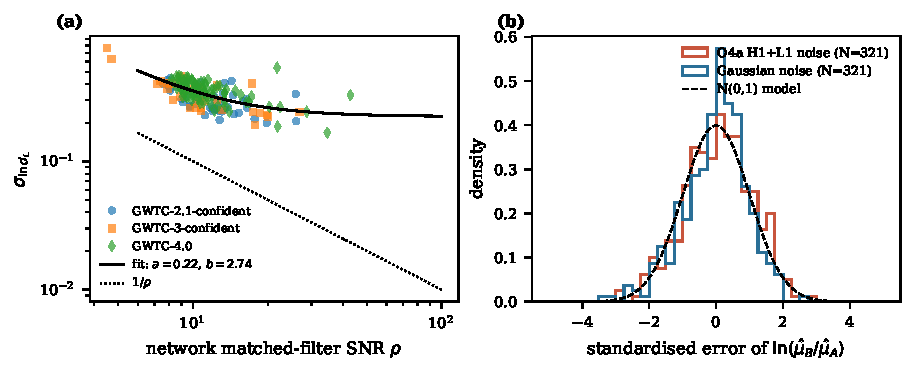
\includegraphics[width=\linewidth]{fig_realdata.pdf}
\caption{Real-data calibration and validation. (a) Log-distance uncertainty versus network matched-filter SNR for 167 confident BBH events in GWTC-1 to GWTC-4.0, with the fitted model used in the simulations. (b) Standardised error of the recovered relative magnification for lensed image pairs injected into public O4a H1/L1 strain and into Gaussian noise with the same PSDs. One glitch-contaminated O4a pair ($z=44.5$) lies outside the plotted range.}
\label{fig:realdata}
\end{figure*}

\section{Inference}
\label{sec:inference}
\subsection{Observables and input sets}
\label{sec:features}
The target is the absolute magnification $\mu_A$ of the image with the larger measured SNR. The image-geometry inputs are the radii of images $A$ and $B$ from the observed lens-light centre, their separation, opening angle and asymmetry, an Einstein-radius proxy $(r_A+r_B)/2$, the number of resolved images and the normalised radii of any additional images, the light axis ratio, and the image position angles relative to the light major axis. The GW inputs are the dimensionless relative magnification $\ln(\hat\mu_B/\hat\mu_A)$ and arrival order ${\rm sign}(\Delta t)$, and the dimensional delay $\ln|\Delta t|$, the two SNRs and the two apparent distances. The follow-up (FU) inputs are the spectroscopic redshifts $z_l$, $z_s$ and the velocity dispersion, $\ln\sigma_v$. Finally, the cosmology estimator $\ln\hat\mu_{\rm cosmo}=2[\ln d_L(\hat z_s)-\ln\hat D_{{\rm app},A}]$ uses the measured source redshift with the Planck18 distance--redshift relation.

Table~\ref{tab:inputsets} lists the combinations of inputs (input sets) that we compare. In their names, GW(ratio) denotes the dimensionless GW observables, $\ln(\hat\mu_B/\hat\mu_A)$ and ${\rm sign}(\Delta t)$; GW(rel) adds the dimensional ones, $\ln|\Delta t|$ and the SNRs; and FU denotes the follow-up redshifts and velocity dispersion. The sets differ in whether they contain a distance scale. Geometry, Geometry+FU, Geometry+GW(ratio) and Geometry+GW(ratio)+FU contain only quantities that are invariant under the mass-sheet transformation and independent of the distance scale (Section~\ref{sec:msd}); we call these sets scale-free. Geometry+GW(rel) adds the delay and the SNRs. With redshifts (Geometry+GW(rel)+FU), an estimator trained on simulations in one cosmology can relate the delay to the time-delay distance and the SNRs to the luminosity distance, so its output depends on that cosmology even though no distance--redshift inversion is supplied explicitly. GW+$z$ and Full contain $\hat\mu_{\rm cosmo}$ explicitly. Distance corrections from the latter four sets are therefore circular for cosmography.

\begin{table}
\centering\papertablestyle
\caption{Input sets. ``Scale-free'' sets are invariant under the mass-sheet transformation and contain no distance scale. FU: follow-up redshifts $z_l$, $z_s$ and velocity dispersion $\sigma_v$.}
\label{tab:inputsets}
\begin{tabularx}{\columnwidth}{@{}lLc@{}}
\toprule
Input set & Inputs & Scale-free \\
\midrule
GW & GW relative magnification, order, delay, SNRs, apparent distances & no \\
GW+$z$ & GW + follow-up + $\hat\mu_{\rm cosmo}$ & no \\
Geometry & image geometry relative to the lens-light centre, light shape & yes \\
Geometry+FU & Geometry + $z_l$, $z_s$, $\sigma_v$ & yes \\
Geometry+GW(ratio) & Geometry + $\ln(\hat\mu_B/\hat\mu_A)$, ${\rm sign}(\Delta t)$ & yes \\
Geometry+GW(ratio)+FU & Geometry+GW(ratio) + $z_l$, $z_s$, $\sigma_v$ & yes \\
Geometry+GW(rel) & Geometry+GW(ratio) + $\ln|\Delta t|$, SNRs & no \\
Geometry+GW(rel)+FU & Geometry+GW(rel) + $z_l$, $z_s$, $\sigma_v$ & no \\
Full & all of the above + apparent distances, $\hat\mu_{\rm cosmo}$ & no \\
\bottomrule
\end{tabularx}
\end{table}

\subsection{Estimators and their uncertainties}
We use two estimators that are constructed (trained) from simulated events. The first is gradient-boosted decision trees in the histogram-based implementation of \textsc{scikit-learn} \citep[hereafter HistGB;][]{pedregosa2011scikit}, trained to predict directly the 5th, 50th and 95th percentiles of $\ln\mu_A$ given the inputs (quantile regression). These percentile estimates need not contain the truth 90 per cent of the time, so we calibrate them with conformalized quantile regression \citep[CQR;][]{romano2019cqr}. On a separate set of simulated events (the calibration set) we compute for each event how far the true value $y_i$ lies outside its predicted interval, $s_i=\max(\hat q_{05,i}-y_i,\,y_i-\hat q_{95,i})$ (negative if inside), and then widen or narrow all intervals by the value of $s$ that 90 per cent of the calibration events do not exceed (the $\lceil(n+1)0.9\rceil$-th smallest of the $n$ values). This guarantees 90 per cent coverage on average over events drawn from the same population as the calibration set, without assuming a Gaussian error distribution. The correction is computed either once for all events (global calibration) or separately within groups of events \citep{vovk2005algorithmic}. The groups are defined either by observed quantities---the number of resolved images or bins of the predicted magnification---or by the true lens family. The latter is a diagnostic only, because the family of a real lens is not known; as an alternative that does not need it, we also calibrate every event on the EPL+shear calibration events alone. Coverage estimates are quoted with binomial uncertainties where they are compared with the nominal level. All simulated events are independent. For each family they are divided at random into 60 per cent for training, 20 per cent for calibration and 20 per cent for testing, on which all results are quoted, and we repeat this with five different random divisions (three for experiments that mix families). Up to 60\,000 selected events per family and scenario are used.

The second estimator is neural posterior estimation \citep[NPE;][]{papamakarios2016fast}, the simulation-based method that has also been used for rapid GW parameter estimation \citep{dax2021neuralposterior}. A neural network---a conditional normalizing flow with spline transformations \citep{durkan2019nsf}, implemented in \textsc{zuko} \citep{rozet2022zuko}---is trained on simulated events to represent the posterior density $p(\ln\mu_A\,|\,\boldsymbol x)$ of the magnification given the inputs $\boldsymbol x$. The posterior median provides the point estimate. We check calibration with the coverage of central intervals at several levels and with the probability integral transform (PIT), the posterior probability below the true value, which is uniformly distributed over events when the posteriors are calibrated.

As a reference without event information we use a prior-only predictor that ignores the event data and returns the percentiles of $\ln\mu_A$ in the training events of the same family. We also evaluate three closed-form estimators: the SIS asymmetry inversion (equation~\ref{eq:sis}), the SIS inversion of the measured relative magnification, and $\hat\mu_{\rm cosmo}$. We report the median relative error $|\hat\mu-\mu|/\mu$, the mean absolute error (MAE) of $\mu_A$, the fraction of events with relative error below 10 per cent, and the interval coverage (the fraction of events whose true value lies inside the interval) and mean log-width.

\section{Results}
\label{sec:results}
\subsection{Selected populations}
Of the simulated lens systems, 51 per cent (SIS) and 42--50 per cent (elliptical families) yield a resolved, detected image pair for ET, and 1.0--1.2 per cent for the O5-like network (Fig.~\ref{fig:population}). ET pairs have median source redshift $z_s\approx2.7$, median delay of about 54\,d and a median brighter-image magnification $\mu_A\approx2.5$. Because the O5-like network must detect both images, its sample is strongly affected by magnification bias. Its pairs lie at lower redshift ($z_s\approx1.9$), are more strongly magnified (median $\mu_A=4.3$--5.2) and contain quadruple-image systems in 33--39 per cent of the elliptical cases, compared with 5--7 per cent for ET. These fractions agree with earlier forecasts of a large quad fraction among magnification-selected lensed BBHs \citep{li2018statistical,wierda2021beyond}. The brighter GW image is the saddle-point image in 14--20 per cent of ET pairs and 28--37 per cent of O5 pairs, because antenna patterns differ between arrival times.

\begin{figure*}
\centering
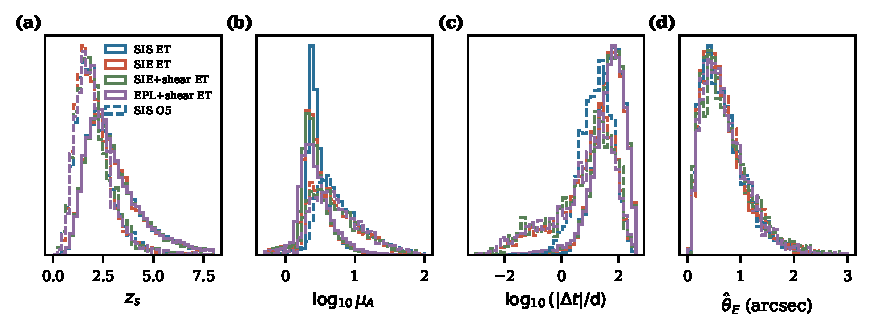
\includegraphics[width=\linewidth]{fig_population.pdf}
\caption{Selected lensed pairs for ET (solid) and the O5-like network (dashed): source redshift, magnification of the brighter GW image, time delay and Einstein-radius proxy, per lens family.}
\label{fig:population}
\end{figure*}

\subsection{Information content of the observables}
\label{sec:information}
Table~\ref{tab:inputs} and Fig.~\ref{fig:inputs} compare the input sets for HistGB estimators trained and tested within each lens family (in-family), and for one NPE trained on all families. Four results stand out.

\emph{Image geometry dominates.} For ET, geometry alone gives median relative errors of 3.2, 7.3, 11.6 and 19.9 per cent for SIS, SIE, SIE+shear and EPL+shear lenses, against 19--32 per cent for the prior-only predictor. Adding the redshifts and velocity dispersion does not help (Geometry+FU), because the image configuration already fixes the dimensionless source position, and $\sigma_v$ with 10 per cent errors constrains the Einstein radius less precisely than the image positions do. The error grows with the number of unobserved lens degrees of freedom: external shear and, above all, the radial slope of the EPL family change the magnification at fixed image configuration.

\emph{The dimensionless GW observables are complementary.} GW data alone give 7.7 per cent for SIS---where the relative magnification fixes $y$ through equation~(\ref{eq:sis})---but 21--26 per cent for the elliptical families. Combined with geometry, the GW relative magnification and arrival order alone (Geometry+GW(ratio)) reduce the SIE+shear error from 11.6 to 10.2 per cent and the EPL+shear error from 19.9 to 18.8 per cent. These inputs are invariant under the mass-sheet transformation and contain no distance scale; this is the scale-free benchmark of our study.

\emph{The delay and the SNRs add information only through the distance scale.} Adding $\ln|\Delta t|$ and the two SNRs without redshifts (Geometry+GW(rel)) changes the errors by at most 0.7 percentage points. With redshifts, however, adding only the delay to Geometry+GW(ratio)+FU improves the EPL+shear error from 18.7 to 16.7 per cent, whereas adding only the SNRs leaves it at 18.2 per cent; all dimensional inputs together give 16.4 per cent. The neural posterior estimator exploits this much more: with Geometry+GW(rel)+FU it reaches 1.7, 5.9, 9.7 and 13.6 per cent, against 3.4, 7.2, 10.6 and 19.8 per cent with the scale-free Geometry+GW(ratio)+FU inputs. The reason is that $\Delta t=(1+z_l)D_{\Delta t}\Delta\phi/c$, so the delay, the redshifts and the simulated cosmology fix the Fermat-potential difference, which constrains the radial slope that geometry leaves free. This information is real only if the distance scale is known. Table~\ref{tab:response} quantifies the dependence. Rescaling all distances by $1/h$ at fixed redshift, as a Hubble constant $h$ times the simulated one would, shifts the Geometry+GW(rel)+FU NPE estimate by ${\rm d}\ln\hat\mu/{\rm d}\ln h=0.69$ for ET and 0.44 for O5, so a 10 per cent error in the assumed $H_0$ biases the magnification by 7 (4) per cent. Scale-free estimators are unaffected to numerical precision. The same NPE estimates respond to an external mass sheet with ${\rm d}\ln\hat\mu/{\rm d}\ln\lambda=-0.69$, whereas the truth scales as $-2$: they partly absorb $\kappa_{\rm ext}$ by misattributing the shorter delay to a steeper lens, but cannot correct for it. HistGB estimates respond less to these transformations (${\rm d}\ln\hat\mu/{\rm d}\ln h=0.13$ for ET), because decision trees predict constant values outside the range of their training data; they are therefore less sensitive to the assumed cosmology but gain correspondingly less from it.

\emph{Known redshift plus cosmology is not competitive on its own.} Inverting the apparent distance with the source redshift gives 41 per cent errors for all families, because the inclination--distance degeneracy calibrated on real events (Section~\ref{sec:realdata}) limits the apparent distance of a single image to $\sigma_{\ln D}\gtrsim0.22$, i.e. $\gtrsim45$ per cent in magnification. Section~\ref{sec:pe} shows that full parameter estimation of both images reduces this floor. Closed-form SIS inversions perform well only when the SIS model is correct and degrade to 21--43 per cent for the elliptical families. A flexible estimator trained on a realistic lens prior is therefore essential.

For the O5-like network all errors are larger (Table~\ref{tab:inputs}b): 10.7, 16.2, 21.9 and 27.9 per cent with geometry and 10.8, 14.8, 18.8 and 25.5 per cent with Geometry+GW(ratio). This is because magnification bias selects highly magnified, near-caustic configurations. The errors stop decreasing above about $10^4$ training events (Fig.~\ref{fig:learning} in Appendix~\ref{app:extra}), so the ET results are not limited by sample size; the smaller O5 samples (1500--3000 per family) cost about 1--2 percentage points.

\begin{table*}
\centering\papertablestyle
\caption{Median relative error $|\hat\mu_A-\mu_A|/\mu_A$ (per cent) of the magnification of image $A$ (larger measured SNR). Parentheses: empirical coverage of the conformal 90 per cent intervals (binomial standard error per division 0.003 for ET and 0.01--0.02 for O5). Top: closed-form estimators. Middle: HistGB trained and tested on the same family, means over five random divisions into training, calibration and test events (standard deviation between divisions below 0.3 percentage points for ET and 1.5 for O5). Bottom: one NPE trained on all four families, with intervals calibrated per true family, which is not possible for real lenses (see Table~\ref{tab:calibration}). Prior only: percentiles of the simulated population, ignoring the event data. FU: follow-up redshifts and velocity dispersion. $^\dagger$Scale-free input sets (Table~\ref{tab:inputsets}).}
\label{tab:inputs}
\textbf{(a) ET}\par\smallskip
\begin{tabular*}{\linewidth}{@{\extracolsep{\fill}}lcccc@{}}
\toprule
Input set & SIS & SIE & SIE+shear & EPL+shear \\
\midrule
SIS analytic (geometry) & 3.3 & 21.0 & 23.8 & 32.9 \\
SIS analytic (GW relative) & 8.7 & 33.0 & 36.5 & 42.5 \\
Known $z_s$ + cosmology & 40.8 & 41.6 & 41.4 & 41.3 \\
\midrule
Prior only$^\dagger$ & 18.7 (0.90) & 24.3 (0.90) & 25.0 (0.90) & 31.6 (0.90) \\
GW & 7.7 (0.90) & 21.4 (0.90) & 21.9 (0.90) & 25.8 (0.90) \\
GW+$z$ & 6.7 (0.90) & 16.9 (0.90) & 17.3 (0.90) & 19.4 (0.90) \\
Geometry$^\dagger$ & 3.2 (0.90) & 7.3 (0.90) & 11.6 (0.90) & 19.9 (0.90) \\
Geometry+FU$^\dagger$ & 3.2 (0.90) & 7.3 (0.90) & 11.6 (0.90) & 19.8 (0.90) \\
Geometry+GW(ratio)$^\dagger$ & 3.0 (0.90) & 6.9 (0.90) & 10.2 (0.90) & 18.8 (0.90) \\
Geometry+GW(ratio)+FU$^\dagger$ & 3.0 (0.90) & 7.0 (0.90) & 10.2 (0.90) & 18.7 (0.90) \\
Geometry+GW(rel) & 2.9 (0.90) & 6.9 (0.90) & 9.9 (0.90) & 18.1 (0.90) \\
Geometry+GW(rel)+FU & 2.7 (0.90) & 6.9 (0.90) & 9.9 (0.90) & 16.4 (0.90) \\
Full & 2.7 (0.90) & 6.9 (0.90) & 10.0 (0.90) & 15.6 (0.90) \\
\midrule
NPE: GW & 9.7 (0.90) & 22.4 (0.90) & 23.9 (0.90) & 27.5 (0.89) \\
NPE: Geometry$^\dagger$ & 3.4 (0.90) & 7.3 (0.90) & 11.9 (0.89) & 20.9 (0.90) \\
NPE: Geometry+GW(ratio)$^\dagger$ & 3.3 (0.90) & 6.8 (0.90) & 10.6 (0.89) & 19.6 (0.89) \\
NPE: Geometry+GW(ratio)+FU$^\dagger$ & 3.4 (0.90) & 7.2 (0.90) & 10.6 (0.89) & 19.8 (0.90) \\
NPE: Geometry+GW(rel) & 3.3 (0.90) & 6.7 (0.90) & 10.2 (0.89) & 18.8 (0.89) \\
NPE: Geometry+GW(rel)+FU & 1.7 (0.89) & 5.9 (0.90) & 9.7 (0.90) & 13.6 (0.90) \\
NPE: Full & 1.8 (0.90) & 6.0 (0.90) & 9.8 (0.90) & 13.8 (0.90) \\
\bottomrule
\end{tabular*}
\par\bigskip\textbf{(b) O5-like network}\par\smallskip
\begin{tabular*}{\linewidth}{@{\extracolsep{\fill}}lcccc@{}}
\toprule
Input set & SIS & SIE & SIE+shear & EPL+shear \\
\midrule
SIS analytic (geometry) & 9.7 & 45.3 & 54.5 & 58.0 \\
SIS analytic (GW relative) & 34.2 & 59.6 & 63.7 & 63.2 \\
Known $z_s$ + cosmology & 46.0 & 49.2 & 53.1 & 50.4 \\
\midrule
Prior only$^\dagger$ & 49.7 (0.91) & 53.5 (0.89) & 52.9 (0.91) & 55.8 (0.90) \\
GW & 29.5 (0.91) & 35.3 (0.90) & 35.4 (0.90) & 34.8 (0.88) \\
GW+$z$ & 19.0 (0.92) & 26.5 (0.89) & 26.8 (0.90) & 29.2 (0.90) \\
Geometry$^\dagger$ & 10.7 (0.90) & 16.2 (0.90) & 21.9 (0.91) & 27.9 (0.88) \\
Geometry+FU$^\dagger$ & 10.7 (0.90) & 16.3 (0.89) & 23.4 (0.91) & 27.9 (0.91) \\
Geometry+GW(ratio)$^\dagger$ & 10.8 (0.90) & 14.8 (0.89) & 18.8 (0.90) & 25.5 (0.90) \\
Geometry+GW(ratio)+FU$^\dagger$ & 10.5 (0.90) & 15.0 (0.89) & 19.4 (0.90) & 25.7 (0.90) \\
Geometry+GW(rel) & 9.9 (0.90) & 15.4 (0.90) & 17.9 (0.90) & 24.8 (0.89) \\
Geometry+GW(rel)+FU & 8.8 (0.91) & 14.7 (0.90) & 18.3 (0.89) & 24.6 (0.90) \\
Full & 8.8 (0.91) & 15.7 (0.90) & 17.7 (0.90) & 24.2 (0.89) \\
\midrule
NPE: GW & 29.3 (0.91) & 36.3 (0.88) & 39.7 (0.89) & 36.6 (0.89) \\
NPE: Geometry$^\dagger$ & 11.3 (0.89) & 14.3 (0.92) & 22.6 (0.90) & 24.8 (0.90) \\
NPE: Geometry+GW(ratio)$^\dagger$ & 10.4 (0.89) & 12.4 (0.90) & 18.0 (0.90) & 27.2 (0.91) \\
NPE: Geometry+GW(ratio)+FU$^\dagger$ & 10.6 (0.89) & 13.1 (0.89) & 17.3 (0.89) & 27.6 (0.91) \\
NPE: Geometry+GW(rel) & 11.4 (0.91) & 12.3 (0.91) & 20.1 (0.90) & 26.2 (0.92) \\
NPE: Geometry+GW(rel)+FU & 7.2 (0.90) & 10.7 (0.91) & 15.0 (0.92) & 21.3 (0.94) \\
NPE: Full & 7.3 (0.91) & 11.1 (0.89) & 15.4 (0.92) & 19.4 (0.93) \\
\bottomrule
\end{tabular*}
\end{table*}

\begin{table*}
\centering\papertablestyle
\caption{Response of the predicted magnification to an external mass sheet ($\lambda=1-\kappa_{\rm ext}$; the truth scales as ${\rm d}\ln\mu/{\rm d}\ln\lambda=-2$) and to a distance scale $1/h$ at fixed redshift (the truth is unchanged). Slopes from $\pm10$ per cent transformations of the fixed test systems. GW(ratio+clock) and GW(ratio+SNR) add only $\ln|\Delta t|$ or only the SNRs to GW(ratio).}
\label{tab:response}
\begin{tabular*}{\linewidth}{@{\extracolsep{\fill}}llcccc@{}}
\toprule
 & & \multicolumn{2}{c}{${\rm d}\ln\hat\mu/{\rm d}\ln\lambda$} & \multicolumn{2}{c}{${\rm d}\ln\hat\mu/{\rm d}\ln h$} \\
Scen. & Input set & HistGB & NPE & HistGB & NPE \\
\midrule
ET & Geometry+GW(ratio)+FU & +0.00 & +0.00 & +0.00 & +0.00 \\
ET & Geometry+GW(rel) & -0.03 & -0.04 & +0.03 & +0.04 \\
ET & Geometry+GW(ratio+clock)+FU & -0.10 & -- & +0.10 & -- \\
ET & Geometry+GW(ratio+SNR)+FU & -0.03 & -- & +0.03 & -- \\
ET & Geometry+GW(rel)+FU & -0.13 & -0.69 & +0.13 & +0.69 \\
ET & Full & -0.21 & -0.71 & +0.21 & +0.71 \\
O5 & Geometry+GW(ratio)+FU & +0.00 & -0.00 & +0.00 & -0.00 \\
O5 & Geometry+GW(rel) & -0.08 & -0.15 & +0.09 & +0.14 \\
O5 & Geometry+GW(ratio+clock)+FU & -0.03 & -- & +0.03 & -- \\
O5 & Geometry+GW(ratio+SNR)+FU & -0.08 & -- & +0.08 & -- \\
O5 & Geometry+GW(rel)+FU & -0.14 & -0.43 & +0.13 & +0.44 \\
O5 & Full & -0.30 & -0.56 & +0.30 & +0.56 \\
\bottomrule
\end{tabular*}
\end{table*}

\begin{figure*}
\centering
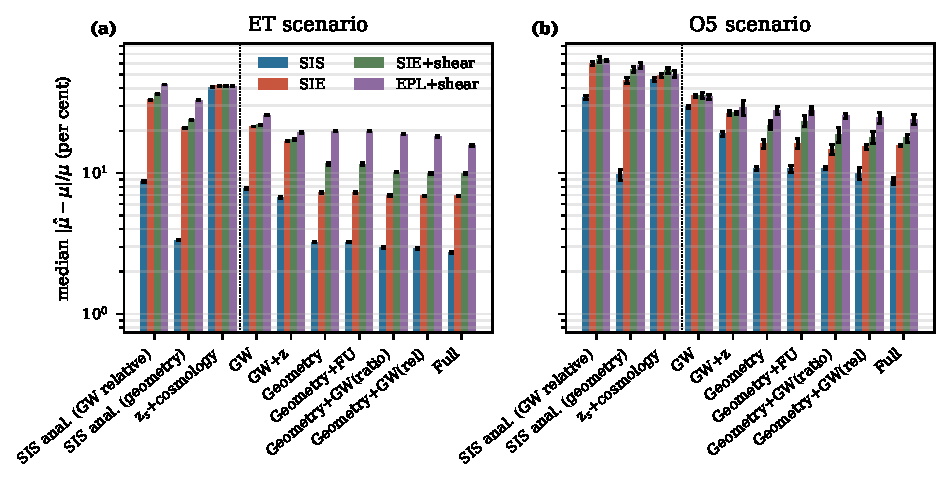
\includegraphics[width=\linewidth]{fig_inputs.pdf}
\caption{Median relative magnification error by input set and lens family (in-family training; error bars: standard deviation over five random divisions). Left of the dotted line: closed-form estimators.}
\label{fig:inputs}
\end{figure*}

\subsection{Near-caustic configurations}
Errors grow rapidly with magnification (Fig.~\ref{fig:tail}). With the scale-free Geometry+GW(ratio) inputs for ET, the median relative error rises from 2--13 per cent at $2<\mu_A<3$ to 10--34 per cent at $5<\mu_A<10$ and 44--57 per cent at $\mu_A>20$. This is the behaviour expected from $\delta\ln\mu=-\operatorname{tr}(A^{-1}\delta A)$: near a fold the same astrometric and model uncertainty produces a magnification error proportional to $\mu$. The rise at $\mu_A<2$ reflects demagnified saddle images that are brighter in SNR only because of the antenna pattern. Intervals calibrated over the whole population contain the truth too rarely in the high-magnification tail (coverage 0.65--0.80 at $10<\mu_A\le20$ and 0.44--0.57 above 20), even though they cover 90 per cent of events overall (Section~\ref{sec:calibration}). Neural posterior estimation with the same scale-free inputs reduces the tail errors only moderately, to 30--46 per cent at $\mu_A>20$. With the delay and redshifts (Geometry+GW(rel)+FU) the tail errors fall to 6--21 per cent, because near a caustic the delay $\Delta t\propto y\,\theta_E^2D_{\Delta t}$ fixes the dimensionless source position once $D_{\Delta t}$ is known. This gain therefore relies on the assumed cosmology and on $\kappa_{\rm ext}=0$.

\begin{figure*}
\centering
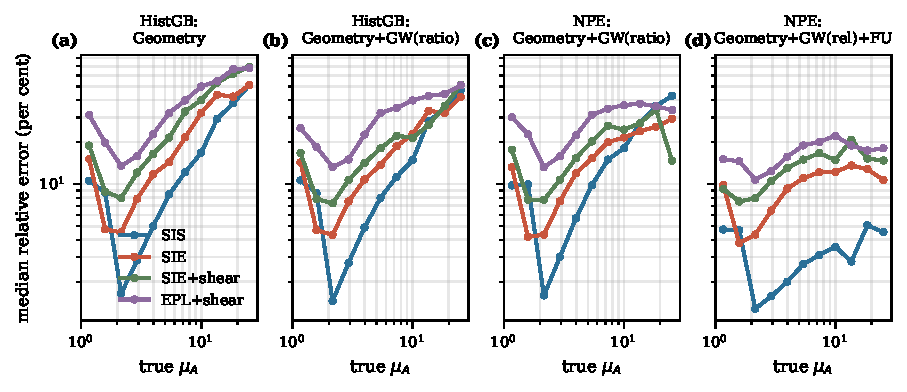
\includegraphics[width=\linewidth]{fig_tail.pdf}
\caption{Median relative error versus true magnification for ET. (a), (b) In-family HistGB models with Geometry and the scale-free Geometry+GW(ratio) inputs (test events of one random division); (c), (d) NPE trained on all families with the scale-free Geometry+GW(ratio) and the scale-dependent Geometry+GW(rel)+FU inputs.}
\label{fig:tail}
\end{figure*}

\subsection{Calibration of the uncertainties}
\label{sec:calibration}
Within a single lens family, CQR intervals achieve the nominal coverage for every input set and both scenarios (0.88--0.92; Table~\ref{tab:inputs}). A single model trained on all four families is almost as accurate as the in-family models (3.4, 7.1, 11.0 and 20.0 per cent with Geometry+GW(ratio) for ET), but a single conformal correction for all families is wrong for each of them. It over-covers SIS and SIE (0.95--0.97) and under-covers EPL+shear (0.75), because the families have different error distributions (Table~\ref{tab:calibration}, Fig.~\ref{fig:coverage}a). Calibrating separately per true family restores 0.90 coverage in every family, but the true family of a real lens is not known. Calibration groups defined by observables do not reproduce it: grouping by the number of images or by the predicted magnification leaves the EPL+shear coverage at 0.75--0.76, because these observables hardly distinguish the families. What does work without a family label is to calibrate on the most flexible family alone. Conformal correction computed on the EPL+shear calibration events gives coverage of at least 0.90 in every family, at the price of 40 per cent wider intervals and over-coverage (0.98--0.99) for the simpler families. The O5 results are similar (Table~\ref{tab:calibration}b).

The conformal guarantee holds on average over the population, or within any group of events defined by \emph{observed} quantities, but not within groups defined by the unobserved true magnification. We therefore also calibrated in-family models in five bins of the \emph{predicted} magnification (Fig.~\ref{fig:coverage}b). By construction this restores 90 per cent coverage in every predicted-magnification bin, but coverage in bins of the true magnification hardly changes: averaged over families it is 0.84, 0.75 and 0.54 for true $\mu_A$ in $(5,10]$, $(10,20]$ and above 20 for ET, against 0.82, 0.73 and 0.51 with a single calibration for all magnifications. Truly near-caustic events are under-covered because, given the measurement noise, they are partly indistinguishable from moderately magnified configurations, and the estimators pull them towards typical magnifications. This is a remaining failure of all calibrated estimators in our study, not one that predicted-magnification calibration solves. Interval widths must therefore be interpreted as conditional on the observables, and analyses that select events by high inferred magnification should account for this regression to the mean.

Neural posterior estimation provides full posteriors. Trained once on all four families with the scale-free Geometry+GW(ratio) inputs for ET, the posterior median reaches 3.3, 6.8, 10.6 and 19.6 per cent, comparable to the in-family HistGB models (3.0, 6.9, 10.2 and 18.8 per cent) without access to the family label. Its raw posteriors are calibrated over the whole population but not per family (coverage 0.94, 0.97, 0.92 and 0.76; Fig.~\ref{fig:coverage}c): the network learns an average error distribution, exactly like the global conformal correction. The same calibration choices apply. Per-true-family recalibration restores 0.89--0.90 in every family; observable groups do not; EPL+shear calibration gives 0.89--0.99. Conformal recalibration adjusts the end points of the 90 per cent interval only and does not by itself certify the rest of the posterior density.

\begin{table*}
\centering\papertablestyle
\caption{Coverage of the 90 per cent intervals per lens family for one model trained on all four families with Geometry+GW(ratio) inputs, for different conformal calibrations. ``Width'' is the mean width of $\ln\mu_A$ intervals over all families. The true-family calibration is a diagnostic only, because the family of a real lens is unknown. HistGB: means over three random divisions; binomial standard errors are below 0.006 (ET) and 0.02 (O5).}
\label{tab:calibration}
\textbf{(a) ET}\par\smallskip
\begin{tabular*}{\linewidth}{@{\extracolsep{\fill}}llccccc@{}}
\toprule
Estimator & Calibration & SIS & SIE & SIE+shear & EPL+shear & width \\
\midrule
HistGB & global & 0.95 & 0.97 & 0.91 & 0.75 & 0.67 \\
HistGB & image multiplicity & 0.95 & 0.97 & 0.92 & 0.76 & 0.67 \\
HistGB & predicted $\mu$ & 0.95 & 0.97 & 0.91 & 0.75 & 0.68 \\
HistGB & EPL+shear only & 0.99 & 0.99 & 0.98 & 0.90 & 0.94 \\
HistGB & true family (diagnostic) & 0.90 & 0.90 & 0.90 & 0.90 & 0.68 \\
\midrule
NPE & global & 0.94 & 0.97 & 0.92 & 0.76 & 0.65 \\
NPE & image multiplicity & 0.94 & 0.97 & 0.92 & 0.76 & 0.65 \\
NPE & predicted $\mu$ & 0.94 & 0.97 & 0.92 & 0.76 & 0.65 \\
NPE & EPL+shear only & 0.99 & 0.99 & 0.98 & 0.89 & 0.91 \\
NPE & true family (diagnostic) & 0.90 & 0.90 & 0.89 & 0.89 & 0.66 \\
\bottomrule
\end{tabular*}
\par\bigskip\textbf{(b) O5-like network}\par\smallskip
\begin{tabular*}{\linewidth}{@{\extracolsep{\fill}}llccccc@{}}
\toprule
Estimator & Calibration & SIS & SIE & SIE+shear & EPL+shear & width \\
\midrule
HistGB & global & 0.92 & 0.92 & 0.87 & 0.81 & 1.13 \\
HistGB & image multiplicity & 0.92 & 0.92 & 0.88 & 0.82 & 1.13 \\
HistGB & predicted $\mu$ & 0.92 & 0.91 & 0.88 & 0.81 & 1.15 \\
HistGB & EPL+shear only & 0.95 & 0.96 & 0.95 & 0.90 & 1.38 \\
HistGB & true family (diagnostic) & 0.88 & 0.90 & 0.88 & 0.90 & 1.11 \\
\midrule
NPE & global & 0.94 & 0.93 & 0.91 & 0.80 & 1.01 \\
NPE & image multiplicity & 0.92 & 0.94 & 0.92 & 0.82 & 1.02 \\
NPE & predicted $\mu$ & 0.94 & 0.94 & 0.91 & 0.80 & 1.02 \\
NPE & EPL+shear only & 0.99 & 0.98 & 0.96 & 0.91 & 1.43 \\
NPE & true family (diagnostic) & 0.89 & 0.90 & 0.90 & 0.91 & 0.98 \\
\bottomrule
\end{tabular*}
\end{table*}

\begin{figure*}
\centering
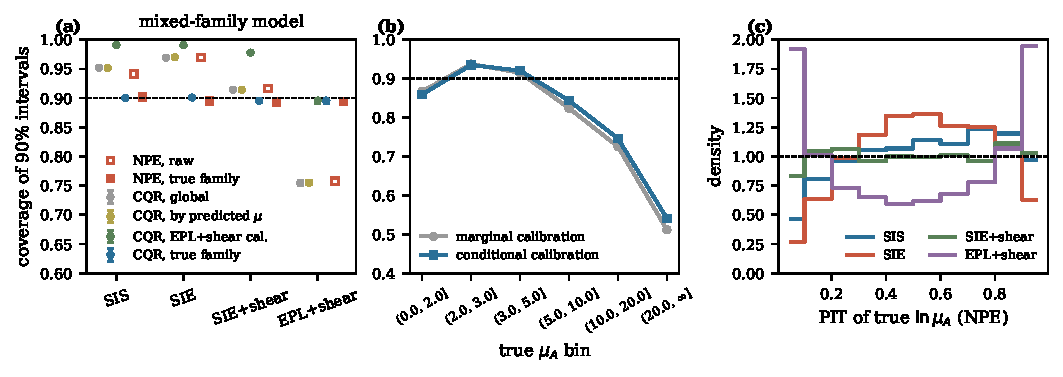
\includegraphics[width=\linewidth]{fig_coverage.pdf}
\caption{Calibration of the 90 per cent intervals for ET (Geometry+GW(ratio) inputs). (a) Coverage per family for a HistGB model trained on all families with global, predicted-magnification, EPL+shear-only and true-family conformal calibration (error bars: scatter between random divisions), and for neural posterior estimation (raw and recalibrated per true family). (b) Coverage in bins of true magnification for a single calibration (``marginal'') and for calibration within bins of predicted magnification (``conditional''); in-family models, mean over families and three random divisions. (c) Histograms of the PIT (posterior probability below the true value) for the NPE; a flat histogram indicates calibrated posteriors.}
\label{fig:coverage}
\end{figure*}

\subsection{Wrong lens-model assumptions}
\label{sec:transfer}
Fig.~\ref{fig:transfer} shows models trained on one family and applied to another. Training on SIS lenses---the default assumption of many lensed-GW forecasts---is the worst choice. Applied to elliptical lenses it gives 21--31 per cent errors with 90 per cent intervals covering only 20--27 per cent of the true values: the SIS prior is confidently wrong. Conversely, the most flexible EPL+shear prior transfers to the simpler families at a moderate accuracy cost (9.4--13.0 per cent instead of 3.0--10.3 per cent in-family) and conservative coverage (0.96--0.98). The SIE and SIE+shear priors transfer well to each other and to SIS, but under-cover EPL+shear lenses (0.48 and 0.61). When SIS, SIE or SIE+shear lenses are omitted from the training set of a model trained on several families, the intervals still cover 91--97 per cent of their true values, at a moderate accuracy cost (for SIS, 3.4 rises to 6.6 per cent), whereas omitting EPL+shear lenses yields 22 per cent errors and coverage 0.55. The radial density slope is thus the dominant lens-model systematic: training sets must include slope variations comparable to those of real lenses, and calibration should use the broadest plausible lens population. This conservative transfer is established only among our four families; real lenses with structure outside the EPL+shear family can still be misdescribed.

\begin{figure*}
\centering
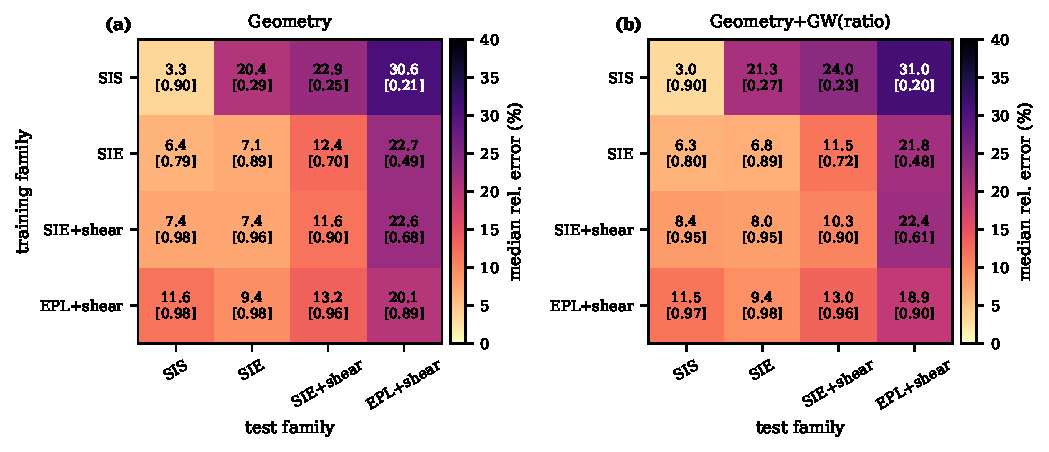
\includegraphics[width=\linewidth]{fig_transfer.pdf}
\caption{Transfer between lens families for ET. Cells give the median relative error (per cent) and, in brackets, the coverage of the 90 per cent intervals, for models trained on the row family and tested on the column family.}
\label{fig:transfer}
\end{figure*}

\subsection{Sky localisation}
The GW relative magnification requires the antenna response of both images, and hence the sky position, polarisation and inclination. With the sky and orientation uncertainties expected for ET alone, the median error of the GW-only SIS estimate is 7.7 per cent; with the sky position known (for example from the identified host galaxy) it falls to 3.9 per cent. Combined with geometry, known sky improves the Geometry+GW(ratio) errors from 10.2 to 8.1 per cent for SIE+shear and from 18.8 to 17.3 per cent for EPL+shear. Host identification therefore also sharpens the GW relative magnification \citep{hannuksela2020localizing,wempe2022lensing}. Because the main benchmark assumes an identified host, its estimated-sky GW errors are conservative; Section~\ref{sec:jointpe} shows that for a single ET detector the known sky also removes occasional wrong solutions of the joint PE.

\subsection{Luminosity distance}
\label{sec:distance}
The magnification correction gives $\hat d_L=\hat D_{{\rm app},A}\,\hat\mu_A^{1/2}$, evaluated event by event, so any correlation between the two estimates is retained. For the scale-free inputs the magnification estimate does not use the apparent distance, so the two errors are independent apart from the shared image SNR. For ET with Geometry+GW(ratio) inputs the magnification contributes a median $|\delta\ln d_L|$ of 1.5, 3.5, 5.1 and 9.5 per cent for SIS, SIE, SIE+shear and EPL+shear. The total median error is 22--24 per cent, almost the same as the 22 per cent obtained with the true magnification (Fig.~\ref{fig:distance}). For O5 the magnification contributes 5--13 per cent, against a total of 27--33 per cent. Under the catalogue-calibrated apparent-distance model, magnification inferred from image geometry is therefore not the limiting factor for the distance of a typical lensed BBH; the exception is a strongly magnified image ($\mu\gtrsim10$). This conclusion depends on the apparent-distance error. The catalogue-calibrated floor $\sigma_{\ln D}\approx0.22$ reflects current detectors, waveform models and the inclination--distance degeneracy; higher harmonics reduce it for third-generation detectors \citep{liu2024harmonics}, and our joint PE gives ET apparent-distance errors about half as large (Section~\ref{sec:jointpe}). With such errors the magnification term is comparable to the GW term for elliptical lenses.

\begin{figure}
\centering
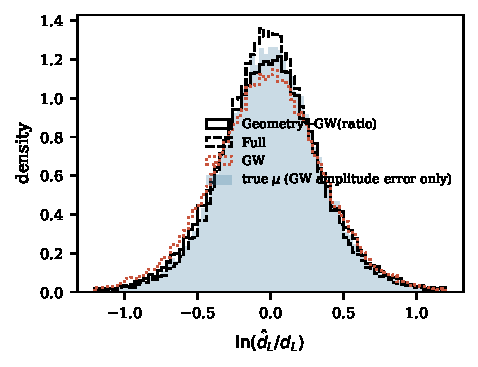
\includegraphics[width=\columnwidth]{fig_distance.pdf}
\caption{Error of the magnification-corrected luminosity distance for ET (all families). The shaded histogram uses the true magnification and shows the GW apparent-distance error alone.}
\label{fig:distance}
\end{figure}

\section{Parameter estimation and Bayesian lens reconstruction}
\label{sec:pe}
The benchmark of Section~\ref{sec:results} uses a simplified, SNR-based model of the GW measurements (Section~\ref{sec:gwmeas}) and estimators trained on simulations. Here we test both ingredients on a random subset of systems, with equal numbers per lens family and scenario: the SNR-based model against joint Bayesian parameter estimation (PE) of both images from simulated detector data (strain), and the trained estimators against conventional Bayesian lens reconstructions that use the same observables and priors, with and without the strain data.

\subsection{Joint parameter estimation of lensed image pairs}
\label{sec:jointpe}
We drew 15 selected systems per lens family and scenario (120 in total) at random from catalogues generated with the same configuration as the benchmark, excluding the lightest detector-frame binaries whose analysis segment would exceed 256\,s. For each system both images were injected into independent stationary Gaussian noise with the A+/AdV (O5-like) or ET-D power spectral densities, using the \textsc{IMRPhenomXHM} waveform with higher harmonics \citep{garciaquiros2020xhm}, the Morse phase of each image and the antenna patterns at each arrival time. We sampled the joint posterior of the shared source parameters (chirp mass, mass ratio, aligned spins, sky position, polarisation, inclination, phase, apparent distance and arrival time of image $A$) and the lensing parameters $\ln(\mu_B/\mu_A)$, the delay and the two Morse indices, with \textsc{bilby} \citep{ashton2019bilby}, the \textsc{dynesty} nested sampler \citep{speagle2020dynesty} and relative binning \citep{zackay2018relbin,krishna2023relbin}, which speeds up the likelihood by expanding each waveform around a reference waveform, here the injected signal. Where the relative-binning log-likelihood exceeds that of the reference waveform by more than 50, which signals a failure of the approximation because the reference lies close to the maximum-likelihood point, we evaluate the exact likelihood instead. We analysed every system twice: with a free sky position, as in a GW-only analysis, and with the sky position fixed to that of the host, which is known to sub-arcsecond precision once the lens system is identified in imaging, as the benchmark assumes. The apparent-distance prior is uniform in volume. We used 150 live points and the acceptance-walk method of \textsc{bilby}, with 30 accepted Markov-chain steps for each new live point. For the free-sky ET posteriors, which have several separated solutions, this is not sufficient (see below), which is one reason we base the comparison with the SNR-based model on the known-sky analyses. Each system has its own noise realisation, fixed by a seed derived from its identifier, so that the GW-only and GW+EM analyses below see identical data. A run takes of order 10--30 CPU hours.

Fig.~\ref{fig:pe} compares the joint-PE posteriors with the SNR-based model of Section~\ref{sec:gwmeas}. With the host sky position, the 90 per cent intervals of $\ln(\mu_B/\mu_A)$ and of the apparent distance of image $A$ contain the truth for 52 and 50 of the 60 ET systems (coverage $0.87\pm0.04$ and $0.83\pm0.05$, binomial errors), and the free-sky O5 intervals for 55 and 53 of 60 ($0.92\pm0.04$ and $0.88\pm0.04$). The probability integral transforms are consistent with uniform (Kolmogorov--Smirnov $p=0.06$ for ET and $0.09$ for O5), and the difference of Morse indices is identified with posterior probability above 0.5 in all ET and in 59 of 60 O5 systems. The PE uncertainties are smaller than those of the SNR-based model: by a factor 0.91 for $\ln(\mu_B/\mu_A)$ in O5 and 0.41 in ET, and by factors 0.67 and 0.44 for $\ln D_{{\rm app},A}$. For ET the SNR-based model is therefore conservative. The joint PE fixes the source parameters that the two images share, and the higher harmonics break part of the inclination--distance degeneracy that dominates the catalogue-calibrated apparent-distance errors, so the median $\sigma_{\ln D}$ is 0.10 for ET rather than 0.24.

Free-sky ET analyses fail in a characteristic way. A single ET site constrains the sky position poorly, and the sky position, the polarisation and the Morse phase of each image are partly degenerate. With 150 live points the sampler often settles on a wrong solution: the median sky offset is $56\degr$, the Morse-index difference is identified in only 82 per cent of systems, and the coverage of $\ln(\mu_B/\mu_A)$ falls to 0.67, in most failures with a likelihood at the true parameters at least as high as at the posterior median, so the sampler has missed the true solution rather than the data disfavouring it. The free-sky ET posteriors are therefore not converged, and the sky position of the host, which is available whenever the lens is identified, is required for ET in practice. O5 analyses, with three detectors, are not affected.

As a test of the complete chain from detector data to magnification, we replaced the simulated relative magnification in the scale-free Geometry+GW(ratio)+FU NPE input by the PE posterior median and kept the per-family conformal calibration of Section~\ref{sec:calibration}. The median relative error of $\mu_A$ is 10.5 per cent for ET with the host sky position (10.8 per cent with the SNR-based model) and 13.8 per cent for O5 (17.8 per cent), with coverage 0.85 and 0.87 for both inputs. The NPE trained with the SNR-based model therefore works with relative magnifications measured by full PE. The SIS intervals under-cover in this subset (0.67--0.73 of 15 systems) for both inputs; these intervals are only a few per cent wide, and the test-set coverage for SIS is nominal, so we attribute this to the small sample.

\begin{figure*}
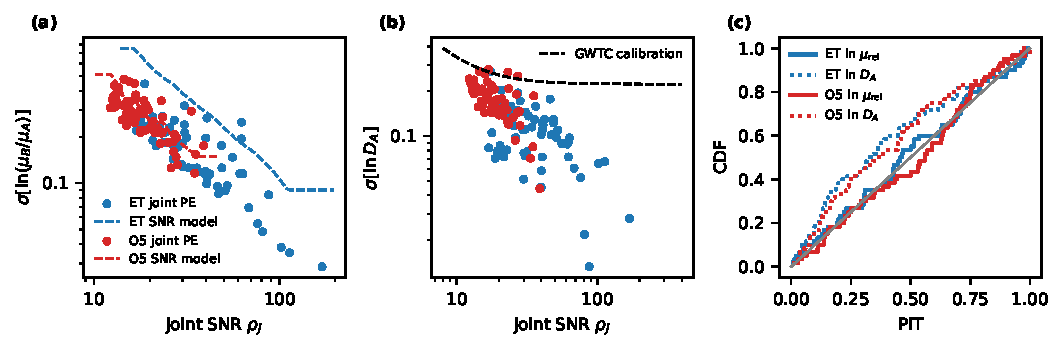
\includegraphics[width=\textwidth]{figures/fig_pe.pdf}
\caption{Joint PE of 120 lensed image pairs from simulated strain. (a) Posterior standard deviation of $\ln(\mu_B/\mu_A)$ versus joint network SNR, with the SNR-based model (dashed). (b) The same for the apparent distance of image $A$, with the GWTC-calibrated error model. (c) Distribution of the probability integral transforms of the truth (diagonal: perfect calibration). ET uses the host sky position, O5 a free sky position.}
\label{fig:pe}
\end{figure*}

\subsection{Bayesian GW+EM lens reconstruction}
\label{sec:gwem}
For the same systems we reconstructed the lens with a conventional likelihood. The lens model is the simulated family (SIS, SIE, SIE+shear or EPL+shear), evaluated with \textsc{lenstronomy}, and its priors are the simulated population distributions: the SLACS-like axis ratio, the log-normal external shear, $\gamma'\sim\mathcal N(2.08,0.15)$ and the $\sigma_v^4$-weighted velocity-dispersion function. The EM likelihood contains the image positions, with the source position integrated out analytically after linearising the lens equation around each observed image, the lens-light axis ratio and orientation, the velocity dispersion through the SIS normalisation, and the lens-light centre. The GW likelihood depends on the lens only through the magnifications, arrival order and Morse indices of the two GW images. We use it in two ways.

\emph{Two-stage analysis.} The joint-PE posterior of Section~\ref{sec:jointpe} is summarised by a Gaussian in $(\ln\mu_B/\mu_A,\ln D_{{\rm app},A})$, after reweighting the samples to remove the distance prior, together with the posterior probabilities of the nine Morse-index combinations. This product is multiplied by the EM likelihood and sampled over the lens parameters only. It is analogous to the effective GW likelihood of \citet{uronen2026silmarel}.

\emph{Full analysis.} The strain likelihood of both images and the EM likelihood are sampled simultaneously, with the source parameters and the lens parameters free. This makes no approximation to the GW likelihood and is the reference for the two-stage analysis. A run takes 20--40 CPU hours; we performed it for 80 of the 120 systems (10 per family and scenario).

Both analyses are run without a cosmology. The GW amplitude then constrains only the relative magnification, and only the arrival order of the delay is used, so they use the information of the scale-free Geometry+GW(ratio)+FU input set, plus the Morse indices, and are directly comparable with the corresponding NPE. As sensitivity tests we also run the two-stage analysis (i) with the EPL+shear model for all families, (ii) with an external convergence $\kappa_{\rm ext}\sim\mathcal N(0,0.025)$, (iii) in a flat $\Lambda$CDM cosmology in which the observed redshifts give $d_L(z_s)$, so that the GW apparent distance measures $|\mu_A|$ and the delay constrains $(1-\kappa_{\rm ext})D_{\Delta t}$, and (iv) with the astrometric error of the GW-source images increased from 0.01 to 0.03 and 0.1\,arcsec, with matching extra scatter in the simulated positions.

Table~\ref{tab:gwem} and Fig.~\ref{fig:gwem} summarise the results. One O5 system is missing from the two-stage analyses because its catalogue entry could not be reproduced exactly from the stored inputs. Coverages of 40--60 systems carry binomial errors of 0.04--0.06.

\emph{Full versus two-stage.} On the 80 systems with both analyses, which see identical noise, the two-stage posterior median of $\ln\mu_A$ differs from the full one by a median $0.15\sigma$ for ET and $0.05\sigma$ for O5, where $\sigma$ is the posterior width, and by more than $1\sigma$ for 10 and 5 per cent of the systems. The 90 per cent intervals have the same width (median ratio 1.02). The largest differences arise when the free-sky ET PE has settled on a wrong sky position (Section~\ref{sec:jointpe}): for one SIE+shear system the free-sky PE places the sky $110\degr$ from the truth and the two-stage $\ln\mu_A$ is off by 3.5, whereas the full analysis, in which the lens model fixes the Morse indices, and the two-stage analysis with the host sky position both recover it. The Gaussian summary of the GW likelihood is therefore adequate, provided the GW posterior itself is converged.

\emph{Bayesian reconstruction versus NPE.} With the host sky position for ET, the two-stage analysis determines $\mu_A$ to a median 8.1 per cent for ET and 13.7 per cent for O5, against 10.5 and 13.8 per cent for the NPE given the same PE relative magnification. Its 90 per cent intervals are 40--45 per cent narrower, but cover the truth less often (0.80 and 0.90 for the two-stage analysis, 0.85 and 0.87 for the NPE, and 0.80 and 0.88 for the full analysis). The NPE, which analyses a new event in seconds once trained, thus reaches the accuracy of a conventional reconstruction within the scatter of these small samples, with calibrated intervals. The Bayesian intervals for ET under-cover by about $2\sigma$, in the full and the two-stage analysis alike (0.75 for the two-stage analysis of free-sky PE, because of the wrong sky solutions). Possible causes are the truncation of the population priors and the linearised image-position likelihood; we have not isolated the cause with these sample sizes.

\emph{Sensitivity tests.} Analysing every system with the EPL+shear model doubles the ET error to 16 per cent (21 per cent for O5), the price of not knowing the lens family, while keeping coverage at 0.80--0.87, in line with the conservative transfer of EPL+shear priors in Section~\ref{sec:transfer}. An external convergence with $\sigma_\kappa=0.025$ hardly changes the scale-free result, because the radial-slope uncertainty dominates. In $\Lambda$CDM, where the observed redshifts turn the GW apparent distance into a magnification measurement and the delay constrains $(1-\kappa_{\rm ext})D_{\Delta t}$, the EPL+shear error falls to 7.3 per cent for ET and 9.8 per cent for O5; this gain is conditional on the assumed cosmology (Section~\ref{sec:discussion}). Increasing the astrometric error of the GW-source images to 0.03\,arcsec leaves the errors within the sample scatter, although the O5 coverage drops to 0.75; at 0.1\,arcsec they roughly double, to 18--19 per cent, and the intervals under-cover (0.66--0.70), which suggests that the linearised image-position likelihood becomes inadequate for larger positional errors. The magnification of a lensed GW image is therefore only as good as the reconstruction of its position in the host.

\begin{table*}
\caption{Bayesian GW+EM reconstruction of $\mu_A$: median relative error and coverage of the 90 per cent interval. Unless noted, the lens model is the true family and no cosmology is assumed. Indented rows modify the known-sky two-stage analysis for ET and the free-sky one for O5. The NPE rows use the scale-free Geometry+GW(ratio)+FU input set.}
\label{tab:gwem}
\begin{tabular*}{\linewidth}{@{\extracolsep{\fill}}lcccccc@{}}
\toprule
 & \multicolumn{3}{c}{ET} & \multicolumn{3}{c}{O5} \\
Analysis & $N$ & err. (\%) & cov. & $N$ & err. (\%) & cov. \\
\midrule
Full (strain + EM), free sky & 40 & 9.6 & 0.80 & 40 & 14.9 & 0.88 \\
Two-stage, free-sky GW PE & 60 & 9.4 & 0.75 & 59 & 13.7 & 0.90 \\
Two-stage, known-sky GW PE & 60 & 8.1 & 0.80 & -- & -- & -- \\
\quad EPL+shear model & 60 & 16.2 & 0.87 & 59 & 20.6 & 0.80 \\
\quad EPL+shear, $\sigma_{\kappa}=0.025$ & 60 & 15.9 & 0.85 & 59 & 21.4 & 0.80 \\
\quad EPL+shear, $\sigma_{\kappa}=0.025$, $\Lambda$CDM & 60 & 7.3 & 0.88 & 59 & 9.8 & 0.93 \\
\quad GW-image astrometry 0.03 arcsec & 60 & 8.9 & 0.85 & 59 & 9.5 & 0.75 \\
\quad GW-image astrometry 0.1 arcsec & 60 & 17.9 & 0.70 & 59 & 18.7 & 0.66 \\
NPE, SNR-model $\mu_B/\mu_A$ & 60 & 10.8 & 0.85 & 60 & 17.8 & 0.87 \\
NPE, joint-PE $\mu_B/\mu_A$ & 60 & 10.5 & 0.85 & 60 & 13.8 & 0.87 \\
\bottomrule
\end{tabular*}
\end{table*}

\begin{figure*}
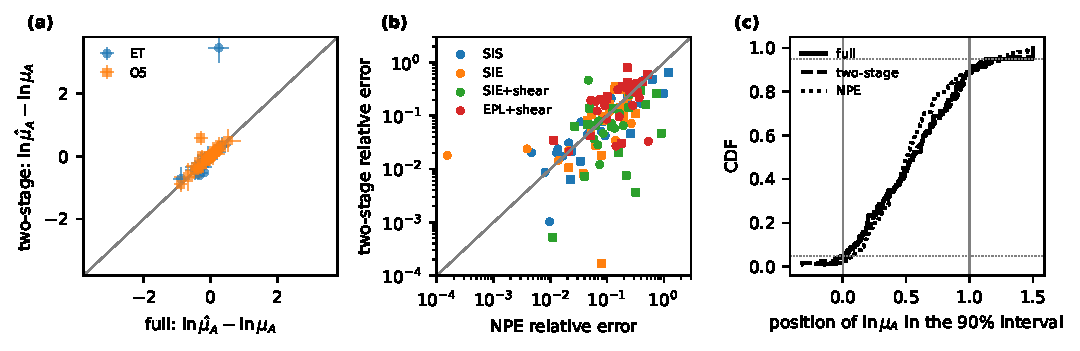
\includegraphics[width=\textwidth]{figures/fig_gwem.pdf}
\caption{Bayesian GW+EM reconstruction. (a) Error of $\ln\mu_A$ from the two-stage versus the full analysis on identical data (free sky). (b) Relative error of the two-stage analysis versus the NPE for the same systems. (c) Distribution of the position of the true $\ln\mu_A$ within the 90 per cent interval (0 and 1 mark its ends) for the full and two-stage analyses and the NPE.}
\label{fig:gwem}
\end{figure*}

\section{Discussion}
\label{sec:discussion}
\subsection{What limits the magnification of a lensed GW image?}
Our results separate five sources of magnification error. (i) \emph{Lens-model freedom at fixed image configuration.} This dominates for realistic lenses: from SIS to SIE, SIE+shear and EPL+shear the geometry-only error grows from 3 to 7, 12 and 20--21 per cent for ET. The radial density slope is the most important unobserved parameter, as expected from the slope--magnification degeneracy familiar from time-delay cosmography. (ii) \emph{Proximity to a caustic.} Errors grow roughly in proportion to $\mu$, so the most strongly magnified---and, for current detectors, most likely to be detected---images are the hardest to correct. (iii) \emph{The GW apparent distance.} Under the catalogue-calibrated error model, the inclination--distance degeneracy limits each image's apparent distance to $\sigma_{\ln D}\approx0.22$, and this dominates the error of the corrected luminosity distance. Joint PE of both images with higher harmonics gives apparent-distance errors smaller by a factor 2.3 for ET and 1.5 for O5 (Section~\ref{sec:jointpe}), so this conclusion depends on the GW analysis and should not be read as a fundamental floor. (iv) \emph{A wrong lens prior.} An estimator trained on an over-simplified lens population produces confidently wrong intervals. This is the most dangerous failure mode, because nothing in the data flags it. (v) \emph{An implicit distance scale.} An estimator that receives the delay or the SNRs together with redshifts gains accuracy by learning the simulated cosmology, and its output then shifts with the assumed $H_0$ (Table~\ref{tab:response}).

These findings suggest a practical strategy for the first lensed BBH with an identified host. Image geometry and the GW relative magnification should be combined with a lens prior that is at least as flexible as an EPL plus external shear with an empirically calibrated slope distribution. Intervals should be calibrated on that flexible prior, because calibration groups defined by observables do not reproduce per-family calibration (Section~\ref{sec:calibration}). Inputs that carry a distance scale should be used only when that scale is part of the analysis rather than an unexamined assumption. Any additional handle on the radial slope---stellar kinematics with a dynamical model, extended-arc modelling of the host, or the GW time delays themselves combined with an independent time-delay distance---should be added, because it targets the dominant error term.

\subsection{Mass-sheet degeneracy and cosmology dependence}
Every result above is conditional on lens populations without an external mass sheet. For estimators that use only scale-free inputs, a sheet with $\lambda\neq1$ multiplies the estimate relative to the truth by exactly $\lambda^2$, which we verified numerically (Table~\ref{tab:response}). For a typical external convergence $|\kappa_{\rm ext}|\lesssim0.05$, this bias of up to 10 per cent in $\mu$ (5 per cent in $d_L$) is comparable to our SIE errors and below those of the EPL family. It would, however, be coherent across a population of lensed events if environments were systematically over- or under-dense. Estimators that use the delay respond to $\lambda$, but only partially (Table~\ref{tab:response}), so they do not remove the bias either. The Bayesian reconstruction makes the trade-off explicit: with $\kappa_{\rm ext}$ free, the scale-free information leaves it unconstrained and the magnification posterior widens accordingly, whereas the delay together with an assumed cosmology constrains $(1-\kappa_{\rm ext})D_{\Delta t}$ (Section~\ref{sec:gwem}). Line-of-sight convergence estimates from galaxy counts or ray tracing, as in time-delay cosmography, can be folded into the prior. Any constraint that uses an assumed cosmology, however, makes the corrected distance circular for cosmography, so the scale-free results are the relevant benchmark for that application.

\subsection{Limitations}
We assumed that the GW images have been associated with each other and with the EM images of an identified host, and that the image positions of the BBH within the host are reconstructed to the stated astrometric precision. The BBH itself is not observed in the EM data, so these positions are the result of an upstream reconstruction of the extended host and the GW information. Its uncertainty may be larger, correlated between images and multimodal, and it must not reuse the GW measurements that enter the magnification inference. Section~\ref{sec:gwem} shows how the magnification degrades with poorer astrometry. A pixel-level reconstruction of lensed hosts with off-centre BBHs, propagated into the GW-source image positions, is needed to replace this assumption; we leave it to future work. The association steps are probabilistic, and the magnification posterior must marginalise over candidate associations and lens reconstructions \citep{hannuksela2020localizing,wempe2022lensing,uronen2026galacticcentres}. The benchmark itself uses the $(2,2)$ mode of an aligned-spin waveform, an SNR-based amplitude model and analytic scalings for the sky and orientation errors. The O4a injections, which recover each image with the exact template, test the relative-amplitude noise prescription in the LIGO detectors only; the joint PE of Section~\ref{sec:jointpe} tests the SNR-based measurement model with higher harmonics and free source parameters, but in Gaussian noise and with aligned spins. Lens populations do not include satellites, line-of-sight structures or redshift evolution of lens properties, and wave-optics effects are negligible for the galaxy-scale lenses considered here but would matter for lower-mass lenses. Each of these simplifications should be relaxed before the method is applied to data.

\section{Conclusions}
\label{sec:conclusions}
We have benchmarked the accuracy and reliability of absolute-magnification inference for strongly lensed GW images from GW and EM observables. The benchmark uses GWTC-4.0 source populations, four galaxy-lens families, O5-like and ET networks, GW distance errors calibrated on 167 GWTC events, and tests of the GW measurement model in public O4a noise and by joint parameter estimation. Our main conclusions are as follows.
\begin{enumerate}
\item Image geometry measured relative to the lens-light centre is the most informative observable. Combined with the GW relative magnification and arrival order---inputs that are invariant under the mass-sheet transformation and contain no distance scale---it determines the magnification of an ET image to a median 3.0, 6.9, 10.2 and 18.8 per cent for SIS, SIE, SIE+shear and EPL+shear lenses (HistGB trained on the correct family; NPE trained on all families gives 3.3--19.6 per cent). For the more magnification-biased O5 sample the errors are 10.8--25.5 per cent.
\item The dimensional time delay and the SNRs add little on their own. With redshifts they reduce the errors further, to 1.7--13.6 per cent for NPE, but only by learning the distance scale of the training cosmology: the inferred magnification then shifts by 0.7 per cent per per cent change in $H_0$. Such estimates are not appropriate for cosmography.
\item GW data alone, or the apparent distance combined with a known source redshift, determine the magnification much less precisely (21--26 and about 41 per cent for realistic lenses), the latter because of the catalogue-calibrated inclination--distance degeneracy.
\item The Gaussian relative-amplitude model holds in real O4a noise for exact-template recovery (standardised scatter 1.02), apart from one glitch-contaminated pair among 321. Joint parameter estimation of 120 image pairs from simulated detector data, with higher harmonics and free source parameters, supports the SNR-based measurement model: with the host sky position the 90 per cent intervals of the relative magnification and the apparent distance contain the truth in 83--92 per cent of systems, and the PE uncertainties are smaller than those of the model. With a free sky position, ET posteriors from a single site have several separated solutions that the sampler does not always find, so the host position is needed in practice.
\item Within a lens family, the calibrated (conformal) 90 per cent intervals contain the truth 90 per cent of the time. An estimator trained on all families needs the family label to be calibrated per family; groups of events defined by observables do not substitute for it. Calibrating on the most flexible (EPL+shear) population gives at least 90 per cent coverage in every family at 40 per cent wider intervals. Near caustics, the intervals contain the truth too rarely for the truly highly magnified images (44--57 per cent for $\mu_A>20$), and calibrating in bins of predicted magnification does not fix this.
\item The lens prior is the dominant systematic. SIS-trained models are confidently wrong for realistic lenses (coverage 20--27 per cent), whereas a flexible EPL+shear prior transfers conservatively to the simpler families we tested. Omitting radial-slope freedom drops interval coverage to 55 per cent.
\item With the catalogue-calibrated apparent-distance errors, the GW apparent distance dominates the error of the corrected luminosity distance for typical lensed BBHs (22--24 per cent total for ET, of which 1.5--9.5 per cent comes from the magnification). Joint parameter estimation with higher harmonics reduces the apparent-distance error by a factor 2.3 for ET (1.5 for O5), so this balance depends on the GW analysis.
\item A conventional Bayesian GW+EM reconstruction with the same information reaches 8.1 (ET) and 13.7 (O5) per cent, comparable to the NPE (10.5 and 13.8 per cent), with 40--45 per cent narrower intervals that contain the truth slightly too rarely for ET. Summarising the GW posterior by a Gaussian in the relative magnification reproduces the full analysis of the detector data (median shift $0.15\sigma$ or less, equal widths) when the GW posterior is converged. The result degrades quickly with the astrometry of the GW-source images, doubling at 0.1\,arcsec.
\end{enumerate}
The code, configuration and real-data calibration are public. The results are conditional on reconstructed GW-source image positions and on the absence of an external mass sheet; pixel-level reconstruction of lensed hosts with off-centre BBHs and line-of-sight convergence are the most important next steps.


\section*{Acknowledgements}
This research has made use of data or software obtained from the Gravitational Wave Open Science Center (gwosc.org), a service of the LIGO Scientific Collaboration, the Virgo Collaboration and KAGRA. We used \textsc{bilby}, \textsc{lalsuite}, \textsc{lenstronomy}, \textsc{astropy}, \textsc{scikit-learn}, \textsc{PyTorch} and \textsc{zuko}.

\section*{Data Availability}
The simulation and analysis code is available at \url{https://github.com/bluejudy151/GW_lensing}. The catalogues can be regenerated with the fixed seeds documented there and are available from the corresponding author on reasonable request. The GW event parameters and O4a strain data are publicly available from GWOSC.

\begin{thebibliography}{99}
\bibitem[Abbott et al.(2021)]{lvk2021o3a}
Abbott R. et al. (LIGO Scientific Collaboration and Virgo Collaboration), 2021, ApJ, 923, 14
\bibitem[Abbott et al.(2023)]{gwosc2023}
Abbott R. et al. (LIGO Scientific Collaboration, Virgo Collaboration and KAGRA Collaboration), 2023, ApJS, 267, 29
\bibitem[Abbott et al.(2024)]{lvk2024o3search}
Abbott R. et al. (LIGO Scientific Collaboration, Virgo Collaboration and KAGRA Collaboration), 2024, ApJ, 970, 191
\bibitem[Ashton et al.(2019)]{ashton2019bilby}
Ashton G. et al., 2019, ApJS, 241, 27
\bibitem[Auger et al.(2010)]{auger2010slacs}
Auger M. W., Treu T., Bolton A. S., Gavazzi R., Koopmans L. V. E., Marshall P. J., Moustakas L. A., Burles S., 2010, ApJ, 724, 511
\bibitem[Birrer \& Amara(2018)]{birrer2018lenstronomy}
Birrer S., Amara A., 2018, Phys. Dark Universe, 22, 189
\bibitem[Birrer et al.(2021)]{birrer2021lenstronomy}
Birrer S. et al., 2021, J. Open Source Softw., 6, 3283
\bibitem[Birrer \& Treu(2019)]{birrer2019astrometry}
Birrer S., Treu T., 2019, MNRAS, 489, 2097
\bibitem[Bolton et al.(2008)]{bolton2008slacs}
Bolton A. S., Burles S., Koopmans L. V. E., Treu T., Gavazzi R., Moustakas L. A., Wayth R., Schlegel D. J., 2008, ApJ, 682, 964
\bibitem[Choi, Park \& Vogeley(2007)]{choi2007vdf}
Choi Y.-Y., Park C., Vogeley M. S., 2007, ApJ, 658, 884
\bibitem[Cutler \& Flanagan(1994)]{cutler1994gravitational}
Cutler C., Flanagan {\'E}. E., 1994, Phys. Rev. D, 49, 2658
\bibitem[Dai \& Venumadhav(2017)]{dai2017morse}
Dai L., Venumadhav T., 2017, preprint (arXiv:1702.04724)
\bibitem[Dax et al.(2021)]{dax2021neuralposterior}
Dax M., Green S. R., Gair J., Macke J. H., Buonanno A., Sch{\"o}lkopf B., 2021, Phys. Rev. Lett., 127, 241103
\bibitem[Durkan et al.(2019)]{durkan2019nsf}
Durkan C., Bekasov A., Murray I., Papamakarios G., 2019, in Advances in Neural Information Processing Systems 32, p. 7511
\bibitem[Ezquiaga et al.(2021)]{ezquiaga2021phase}
Ezquiaga J. M., Holz D. E., Hu W., Lagos M., Wald R. M., 2021, Phys. Rev. D, 103, 064047
\bibitem[Falco, Gorenstein \& Shapiro(1985)]{falco1985msd}
Falco E. E., Gorenstein M. V., Shapiro I. I., 1985, ApJ, 289, L1
\bibitem[Garc{\'\i}a-Quir{\'o}s et al.(2020)]{garciaquiros2020xhm}
Garc{\'\i}a-Quir{\'o}s C. et al., 2020, Phys. Rev. D, 102, 064002
\bibitem[Haris et al.(2018)]{haris2018identifying}
Haris K., Mehta A. K., Kumar S., Venumadhav T., Ajith P., 2018, preprint (arXiv:1807.07062)
\bibitem[Hannuksela et al.(2019)]{hannuksela2019search}
Hannuksela O. A., Haris K., Ng K. K. Y., Kumar S., Mehta A. K., Keitel D., Li T. G. F., Ajith P., 2019, ApJ, 874, L2
\bibitem[Hannuksela et al.(2020)]{hannuksela2020localizing}
Hannuksela O. A., Collett T. E., {\c{C}}al{\i}{\c{s}}kan M., Li T. G. F., 2020, MNRAS, 498, 3395
\bibitem[Hild et al.(2011)]{hild2011etd}
Hild S. et al., 2011, Class. Quantum Grav., 28, 094013
\bibitem[Janquart et al.(2023)]{janquart2023golum}
Janquart J., Haris K., Hannuksela O. A., Van Den Broeck C., 2023, MNRAS, 526, 3088
\bibitem[Krishna et al.(2023)]{krishna2023relbin}
Krishna K. et al., 2023, preprint (arXiv:2312.06009)
\bibitem[Li et al.(2018)]{li2018statistical}
Li S.-S., Mao S., Zhao Y., Lu Y., 2018, MNRAS, 476, 2220
\bibitem[Liu et al.(2024)]{liu2024harmonics}
Liu J.-D., Han W.-B., Yun Q., Yang S.-C., 2024, preprint (arXiv:2405.11279)
\bibitem[Liao et al.(2017)]{liao2017precision}
Liao K., Fan X.-L., Ding X., Biesiada M., Zhu Z.-H., 2017, Nat. Commun., 8, 1148
\bibitem[LIGO Scientific Collaboration et al.(2025a)]{lvk2025gwtc4}
LIGO Scientific Collaboration, Virgo Collaboration, KAGRA Collaboration, 2025a, preprint (arXiv:2508.18082)
\bibitem[LIGO Scientific Collaboration et al.(2025b)]{lvk2025gwtc4pop}
LIGO Scientific Collaboration, Virgo Collaboration, KAGRA Collaboration, 2025b, preprint (arXiv:2508.18083)
\bibitem[LIGO Scientific Collaboration et al.(2025c)]{lvk2025gwtc4lensing}
LIGO Scientific Collaboration, Virgo Collaboration, KAGRA Collaboration, 2025c, preprint (arXiv:2512.16347)
\bibitem[Lo \& Maga{\~n}a Hernandez(2023)]{lo2023bayesian}
Lo R. K. L., Maga{\~n}a Hernandez I., 2023, Phys. Rev. D, 107, 123015
\bibitem[Madau \& Dickinson(2014)]{madau2014cosmic}
Madau P., Dickinson M., 2014, ARA\&A, 52, 415
\bibitem[Meneghetti et al.(2017)]{meneghetti2017ff}
Meneghetti M. et al., 2017, MNRAS, 472, 3177
\bibitem[Ng et al.(2018)]{ng2018rates}
Ng K. K. Y., Wong K. W. K., Broadhurst T., Li T. G. F., 2018, Phys. Rev. D, 97, 023012
\bibitem[Oguri(2018)]{oguri2018distribution}
Oguri M., 2018, MNRAS, 480, 3842
\bibitem[Oguri(2019)]{oguri2019review}
Oguri M., 2019, Rep. Prog. Phys., 82, 126901
\bibitem[Papamakarios \& Murray(2016)]{papamakarios2016fast}
Papamakarios G., Murray I., 2016, in Advances in Neural Information Processing Systems 29, p. 1028
\bibitem[Pedregosa et al.(2011)]{pedregosa2011scikit}
Pedregosa F. et al., 2011, J. Mach. Learn. Res., 12, 2825
\bibitem[Planck Collaboration(2020)]{planck2020cosmology}
Planck Collaboration, 2020, A\&A, 641, A6
\bibitem[Poon et al.(2025)]{poon2025degeneracy}
Poon J. S. C., Rinaldi S., Janquart J., Narola H., Hannuksela O. A., 2025, MNRAS, 536, 2212
\bibitem[Pratten et al.(2020)]{pratten2020xas}
Pratten G., Husa S., Garc{\'i}a-Quir{\'o}s C., Colleoni M., Ramos-Buades A., Estell{\'e}s H., Jaume R., 2020, Phys. Rev. D, 102, 064001
\bibitem[Romano, Patterson \& Cand{\`e}s(2019)]{romano2019cqr}
Romano Y., Patterson E., Cand{\`e}s E., 2019, in Advances in Neural Information Processing Systems 32, p. 3543
\bibitem[Rozet et al.(2022)]{rozet2022zuko}
Rozet F. et al., 2022, zuko: Normalizing flows in PyTorch, Zenodo, doi:10.5281/zenodo.7625672
\bibitem[Schneider, Ehlers \& Falco(1992)]{schneider1992gravitationallenses}
Schneider P., Ehlers J., Falco E. E., 1992, Gravitational Lenses. Springer-Verlag, Berlin
\bibitem[Schneider \& Sluse(2013)]{schneider2013msd}
Schneider P., Sluse D., 2013, A\&A, 559, A37
\bibitem[Smith et al.(2023)]{smith2023discovering}
Smith G. P. et al., 2023, MNRAS, 520, 702
\bibitem[Speagle(2020)]{speagle2020dynesty}
Speagle J. S., 2020, MNRAS, 493, 3132
\bibitem[Takahashi \& Nakamura(2003)]{takahashi2003waveeffects}
Takahashi R., Nakamura T., 2003, ApJ, 595, 1039
\bibitem[Tessore \& Metcalf(2015)]{tessore2015epl}
Tessore N., Metcalf R. B., 2015, A\&A, 580, A79
\bibitem[Turner, Ostriker \& Gott(1984)]{turner1984statistics}
Turner E. L., Ostriker J. P., Gott J. R., 1984, ApJ, 284, 1
\bibitem[Uronen et al.(2026a)]{uronen2026silmarel}
Uronen L. et al., 2026a, preprint (arXiv:2603.09794)
\bibitem[Uronen et al.(2026b)]{uronen2026galacticcentres}
Uronen L., Li T., He Q., Janquart J., Collett T., Koopmans L. V. E., Hannuksela O., 2026b, preprint (arXiv:2609.10285)
\bibitem[Vovk, Gammerman \& Shafer(2005)]{vovk2005algorithmic}
Vovk V., Gammerman A., Shafer G., 2005, Algorithmic Learning in a Random World. Springer, New York
\bibitem[Wempe et al.(2024)]{wempe2022lensing}
Wempe E., Koopmans L. V. E., Wierda A. R. A. C., Hannuksela O. A., Van Den Broeck C., 2024, MNRAS, 530, 3368
\bibitem[Wierda et al.(2021)]{wierda2021beyond}
Wierda A. R. A. C., Wempe E., Hannuksela O. A., Koopmans L. V. E., Van Den Broeck C., 2021, ApJ, 921, 154
\bibitem[Zackay, Dai \& Venumadhav(2018)]{zackay2018relbin}
Zackay B., Dai L., Venumadhav T., 2018, preprint (arXiv:1806.08792)
\end{thebibliography}


\appendix
\section{Frame invariance and an information leak in a fixed-origin simulation}
\label{app:leak}
Simulations frequently place the lens at the coordinate origin. If absolute image coordinates are then given to a trained estimator, it can measure the image radii from the exact lens centre and so bypass the error of the measured centre: the inputs contain information that real data do not provide. We quantified this effect on an earlier, smaller benchmark of 2500 selected SIS events (ET-D, $0.05<z_s<1.5$) in which the true centre was fixed at the origin and the inputs contained absolute image and centre coordinates. With otherwise identical HistGB settings and ten random divisions into training, calibration and test events (1750/375/375), replacing the absolute coordinates by translation-invariant inputs raised the MAE of the geometry-only estimate from $0.193\pm0.038$ to $0.270\pm0.040$, and that with all inputs from $0.207\pm0.041$ to $0.239\pm0.036$. A Bayesian SIS posterior from the image coordinates, marginalised over the unknown centre, attains MAE $0.243\pm0.032$ on the same events: it beats the corrected estimator, as it should for a correct lens model, whereas the estimator with absolute coordinates appeared to beat it. In the same earlier study, images in the non-SIS benchmark had been ordered by their true magnification, which reveals the target whenever more than two images exist. All results in this paper use a random true centre and frame rotation, inputs that are invariant under translations and rotations, and images ordered by measured SNR.

\section{Additional results}
\label{app:extra}
Fig.~\ref{fig:learning} shows the median relative error as a function of the number of training events for SIS and SIE+shear lenses (ET). The errors stop decreasing above $\sim10^4$ events. The results are therefore not limited by the size of the ET training sets (36\,000 events per family), while the O5 samples (900--1800 training events per family) lose about 1--2 percentage points relative to the asymptotic accuracy.

\begin{figure}
\centering
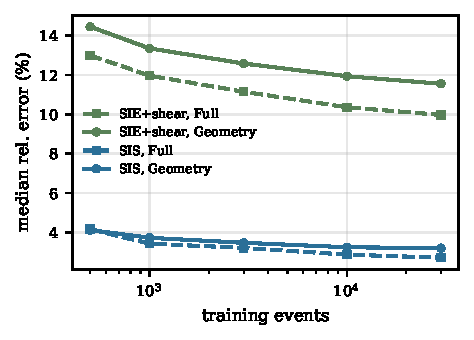
\includegraphics[width=\columnwidth]{fig_learning.pdf}
\caption{Median relative error of $\mu_A$ versus the number of training events for ET.}
\label{fig:learning}
\end{figure}



\bsp
\label{lastpage}
\end{document}
